\documentclass[12pt]{article}

\usepackage{fullpage}
\usepackage{graphicx, rotating, booktabs} 
\usepackage{times} 
\usepackage{natbib} 
\usepackage{indentfirst} 
\usepackage{setspace}
\usepackage{grffile} 
\usepackage{hyperref}
\usepackage{adjustbox}
\usepackage{amsmath}
\usepackage{siunitx}
\usepackage{multirow}
\setcitestyle{aysep{}}


\singlespace
\title{\textbf{Public Attitudes Towards Military Alliances}}
\author{Joshua Alley \\
Postdoctoral Research Associate \\
University of Virginia.\thanks{Thanks to Erik Lin-Greenberg, Philip Potter, Justin Schon and Todd Sechser, as well as participants in the Democratic Statecraft Lab Research incubator, the Lansing B. Lee/Bankard Seminar in Global Politics, 2020 Annual Meeting of the Peace Science Society and 2021 Meeting of the International Studies Association for helpful comments. Preregistration files for this study are hosted in an OSF repository at https://osf.io/g28zs.} \\
jkalley@virginia.edu
}
\date{\today}

\bibliographystyle{apsr}

\begin{document}

\maketitle 

\doublespace 

\begin{abstract}
Why do Americans support or oppose military alliances? 
Although public backing for promises to defend other countries shapes the credibility and durability of U.S. alliance commitments, we know little about the foundations of public opinion towards alliances.
In particular, existing survey evidence cannot determine whether elites lead public alliance attitudes or pander to public opinion. 
In this article, I answer this puzzle about the sources of alliance attitudes by showing how different foreign policy dispositions shape individual responses to cues from copartisan elites. 
I then use two conjoint survey experiments to assess how elite cues shape public attitudes towards forming or maintaining international alliances.  
I find that elite cues often influence alliance attitudes, but that important subsets of both parties are unresponsive to elite cues. 
There is a partisan asymmetry in alliance attitudes, as staunch alliance supporters in the Democratic party are unresponsive to elite cues, while consistent alliance skeptics in the Republican party pay less heed to elites.  
The results imply that elites influence public opinion towards military alliances, but foreign policy dispositions constrain their impact.  
\end{abstract}


\newpage 


\section{Introduction}

% lay out the question
What determines U.S. public opinion towards military alliances? 
Despite the importance of public attitudes for forming and upholding U.S. alliances, we do not know why the public supports or opposes alliance commitments. 
Most existing evidence on this question comes from opinion polls measuring public sentiment towards salient alliances like the North Atlantic Treaty Organization (NATO).
These polls can describe aggregate support and show changes over time, but they do not explain why individuals express particular opinions. 


% puzzle
Descriptive polling data is insufficient because alliance attitudes reflect a longstanding puzzle about who leads or follows in scholarship on public opinion in foreign policy.
Whether elites lead or follow public opinion is a crucial issue for alliance attitudes. 
On the one hand, elites have ample opportunity to lead public opinion on alliances, given limited public information and interest \citep{Canes-Wrone2006, Druckman2014}.
On the other, leaders often pander to existing public attitudes \citep{Barberaetal2019, HagerHilbig2020}.\footnote{See the following article for an illustration of this question in U.S. attitudes towards NATO: \url{https://fivethirtyeight.com/features/is-trump-fueling-republicans-concerns-about-nato-or-echoing-them/}.}
Partisanship, foreign policy dispositions, and economic interests all give structure to public foreign policy attitudes that could limit the influence of elites \citep{Holsti1992, PageShapiro1992, KertzerZeitzoff2017}


% contribution
In this paper, I unpack elite leadership in alliance attitudes. 
To do so, I identify responses to elite cues by individuals in each party with different foreign policy dispositions.
I scrutinize whether elites lead or pander to public opinion by assessing whether elite cues impact support regardless of individual predispositions to support alliances from isolationism and hawkishness.  
Isolationists are predisposed to oppose alliances, while hawks are likely to back alliance participation. 
While most individuals in both parties respond to co-partisan elite cues, the strongest alliance supporters in the Democratic party hold more rigid alliance attitudes, as do the greatest alliance skeptics in the Republican party. 
Therefore, elites have ample scope to lead public alliance attitudes, but their influence faces some constraints. 


% Importance part 1: public opinion undergirds alliance com in democ
In addition to providing new insight into the puzzle of who leads whom, there are three reasons that understanding U.S. public opinion towards alliances is worthwhile. 
To start, public support is at the heart of debates over the reliability and durability of democratic commitments.\footnote{Public opinion is important, but it is not deterministic. \citet{Kreps2010} notes that public disapproval may not hinder coalition warfare, especially when elite consensus favors fighting.}
For example, NATO leaders often feared that changing public attitudes would undermine the alliance \citep{Sayle2019}.   
If public opinion towards alliances depends on individual concerns and alliance characteristics, this may lead to stable attitudes and reliable commitments \citep{Gaubatz1996}.
If elite cues are more consequential, then elite alliance skeptics can bring the public along, leading to cycles that hinder democratic reliability \citep{GartzkeGleditsch2004}.


% importance part 2: practical relevance- US role in world. 
Why the public supports or opposes alliances also speaks to the consequences of a prominent debate in U.S. foreign policy. 
Two competing visions of future U.S. foreign policy depend heavily on alliances. 
One view believes that the United States should reduce its alliance commitments as part of a more restrained grand strategy \citep{Preble2009, Posen2014}.
The other argues that continued deep engagement through alliances is the best way to promote U.S. security and prosperity \citep{Brooksetal2013, BrandsFeaver2017}. 
If elite cues drive public opinion, policymakers and political leaders have substantial latitude to change U.S. alliance commitments. 
But if public opinion towards alliances is based on individual concerns and alliance characteristics, elites risk public disapproval if they undermine popular alliances.  
For example, some observers feared that Donald Trump's strident rhetoric would undermine domestic support for alliances.
Yet U.S. public approval of alliances like NATO remained steady during the Trump administration \citep{PewNATO2020}. 


% importance part 3: WHY support international cooperation, not just consequences of international institutions
In addition to its practical importance, this study fills a gap in international institutions scholarship. 
Scholars are more likely to study how international institutions affect public attitudes (e.g. \citep{KayaWalker2014, Greenhill2020}), than scrutinize the sources of public attitudes towards international institutions themselves. 
Other studies use observational survey data to examine public opinion towards international cooperation such as multilateral financial institutions \citep{Edwards2009} or the United Nations \citep{Torgler2008, DellmuthTallberg2015}. 
There is little experimental evidence of why the public supports or opposes alliances.
In one study of public opinion and military alliances, \citet{TomzWeeks2021} show that the presence of an alliance increases public support for foreign military intervention. 
\citet{Chuetal2021} explore how values and interest based elite cues shape public attitudes towards alliance maintenance. 
I build on these works with more general experiments on alliance formation and maintenance. 


% survey on NATO, etc don't get at it
There is therefore little evidence to explain why individuals support forming and maintaining military alliances. 
Most existing evidence comes from tracking changes in public opinion over time across surveys.
This gives useful descriptive data, but it does not provide causal evidence.


% Assess w/ a survey experiment
I use two conjoint survey experiments to assess the sources of public opinion towards alliances. 
Conjoint experiments randomize multiple alliance characteristics and elite cues, so this tool is well-suited to assessing the relative weight of different factors \citep{Hainmuelleretal2014}.
Unlike in observational data, in the context of an experiment that randomly assigns elite cues, I can use information on foreign policy dispositions within parties to distinguish who leads and who follows. 
The first study asks individuals to rate five hypothetical new alliance commitments and support or oppose alliance formation.
The second asks respondents to rate five hypothetical existing commitments and support or oppose alliance maintenance. 


% how address puzzle
In my analysis, I address the puzzle of whether elites lead or pander to public opinion towards alliances. 
To disentangle these relationships, I start by estimating the unconditional average marginal component effects of different elite cues and alliance attributes.
I then examine how partisanship and foreign policy dispositions shape individual responses to elite cues and alliance characteristics. 


% findings
In nationally representative survey experiments on alliance formation and maintenance, I find that the impact of elite cues and baseline alliance support depend on partisanship and foreign policy dispositions. 
Hawkish individuals in both parties often support alliance participation, even if they also hold isolationist views.
The implications of hawkishness vary across parties, however. 
Particular groups of Democrats and Republicans hold such strong alliance attitudes that they are unresponsive to elite cues.
Hawkish and isolationist Democrats express consistent support for alliance participation.
Dovish and isolationist Republicans often oppose alliance participation. 
Other partisans shift their alliance attitudes in response to co-partisan elite cues. 
As a result, Republicans can lead the most likely alliance supporters in their party, while Democrats can lead likely alliance skeptics. 
This implies that if elites pander to the strongest alliance attitudes in their party, they could lead many other party members to shift their attitudes in competing directions. 


% partisan differences in democracy, region
I also find partisan differences in how individuals weigh the impact of allied democracy. 
Democrats consistently back alliances with other democracies. 
Isolationist Republicans place far less emphasis on allied regime type. 


% differences between formation and mainteance
Last, I find that alliance formation and maintenance command different support levels.
Even with elite opposition, upholding existing alliances almost always retains majority support. 
On the other hand, elite cues can determine whether forming a new alliance has majority or minority support. 
Therefore, elites have more influence over expanding U.S. obligations, relative to changing existing commitments. 


% Implications
The results imply that elites have substantial latitude to shape public attitudes towards alliances. 
Elite influence on alliance attitudes does not reach all partisans equally, however, as foreign policy dispositions make some individuals less responsive. 
Therefore, elite leadership has substantial influence, but important subsets of both parties hold more rigid attitudes.


These findings speak directly to the future of U.S. alliance politics. 
Although elite cues can weaken public support for U.S. alliances, they are unlikely to shift alliance attitudes towards majority opposition, given high baseline support for alliance maintenance.
Should U.S. allies become less democratic, however, elite opposition could stoke enough public disapproval to endangers an alliance.
Bipartisan opposition to alliances would also probably generate enough public support for leaders to withdraw from an alliance with little public disapproval.  


% Try it w/o the plan of paper for flow. 


\section{Who Leads Alliance Attitudes?}

Public opinion has a critical role in democratic foreign policy and alliance politics.
Public approval guides decisions about military force and whether to intervene in foreign conflicts \citep{Tomzetal2020, LinGreenberg2021}. 
In democracies, anticipation of public disapproval of treaty violation encourages conditional promises of military support \citep{Chibaetal2015, FjelstulReiter2019}. 
Moreover, public attitudes have a key role in disputes about the reliability of democratic alliances \citep{Gaubatz1996, GartzkeGleditsch2004}. 
Last, policymakers pay careful attention to public support for alliances \citep{Sayle2019}. 


% NATO example to bring out the puzzle
There is also meaningful variation in pubic opinion towards military alliances. 
\autoref{fig:nato-op-time} plots the percentage of respondents supporting NATO in 59 surveys from 1974 to 2020.\footnote{These surveys ask respondents to assess NATO in many ways. I consider favorable opinions, feeling thermometer ratings of 50 or higher, and support for increasing or maintaining U.S. commitment as indicators of support for NATO.} 
NATO generally commands majority support in public opinion, but average support has fallen since 2000. 
Although the general patterns are clear, this does not explain why individuals support alliances and support changes over time. 


\begin{figure}
	\centering
		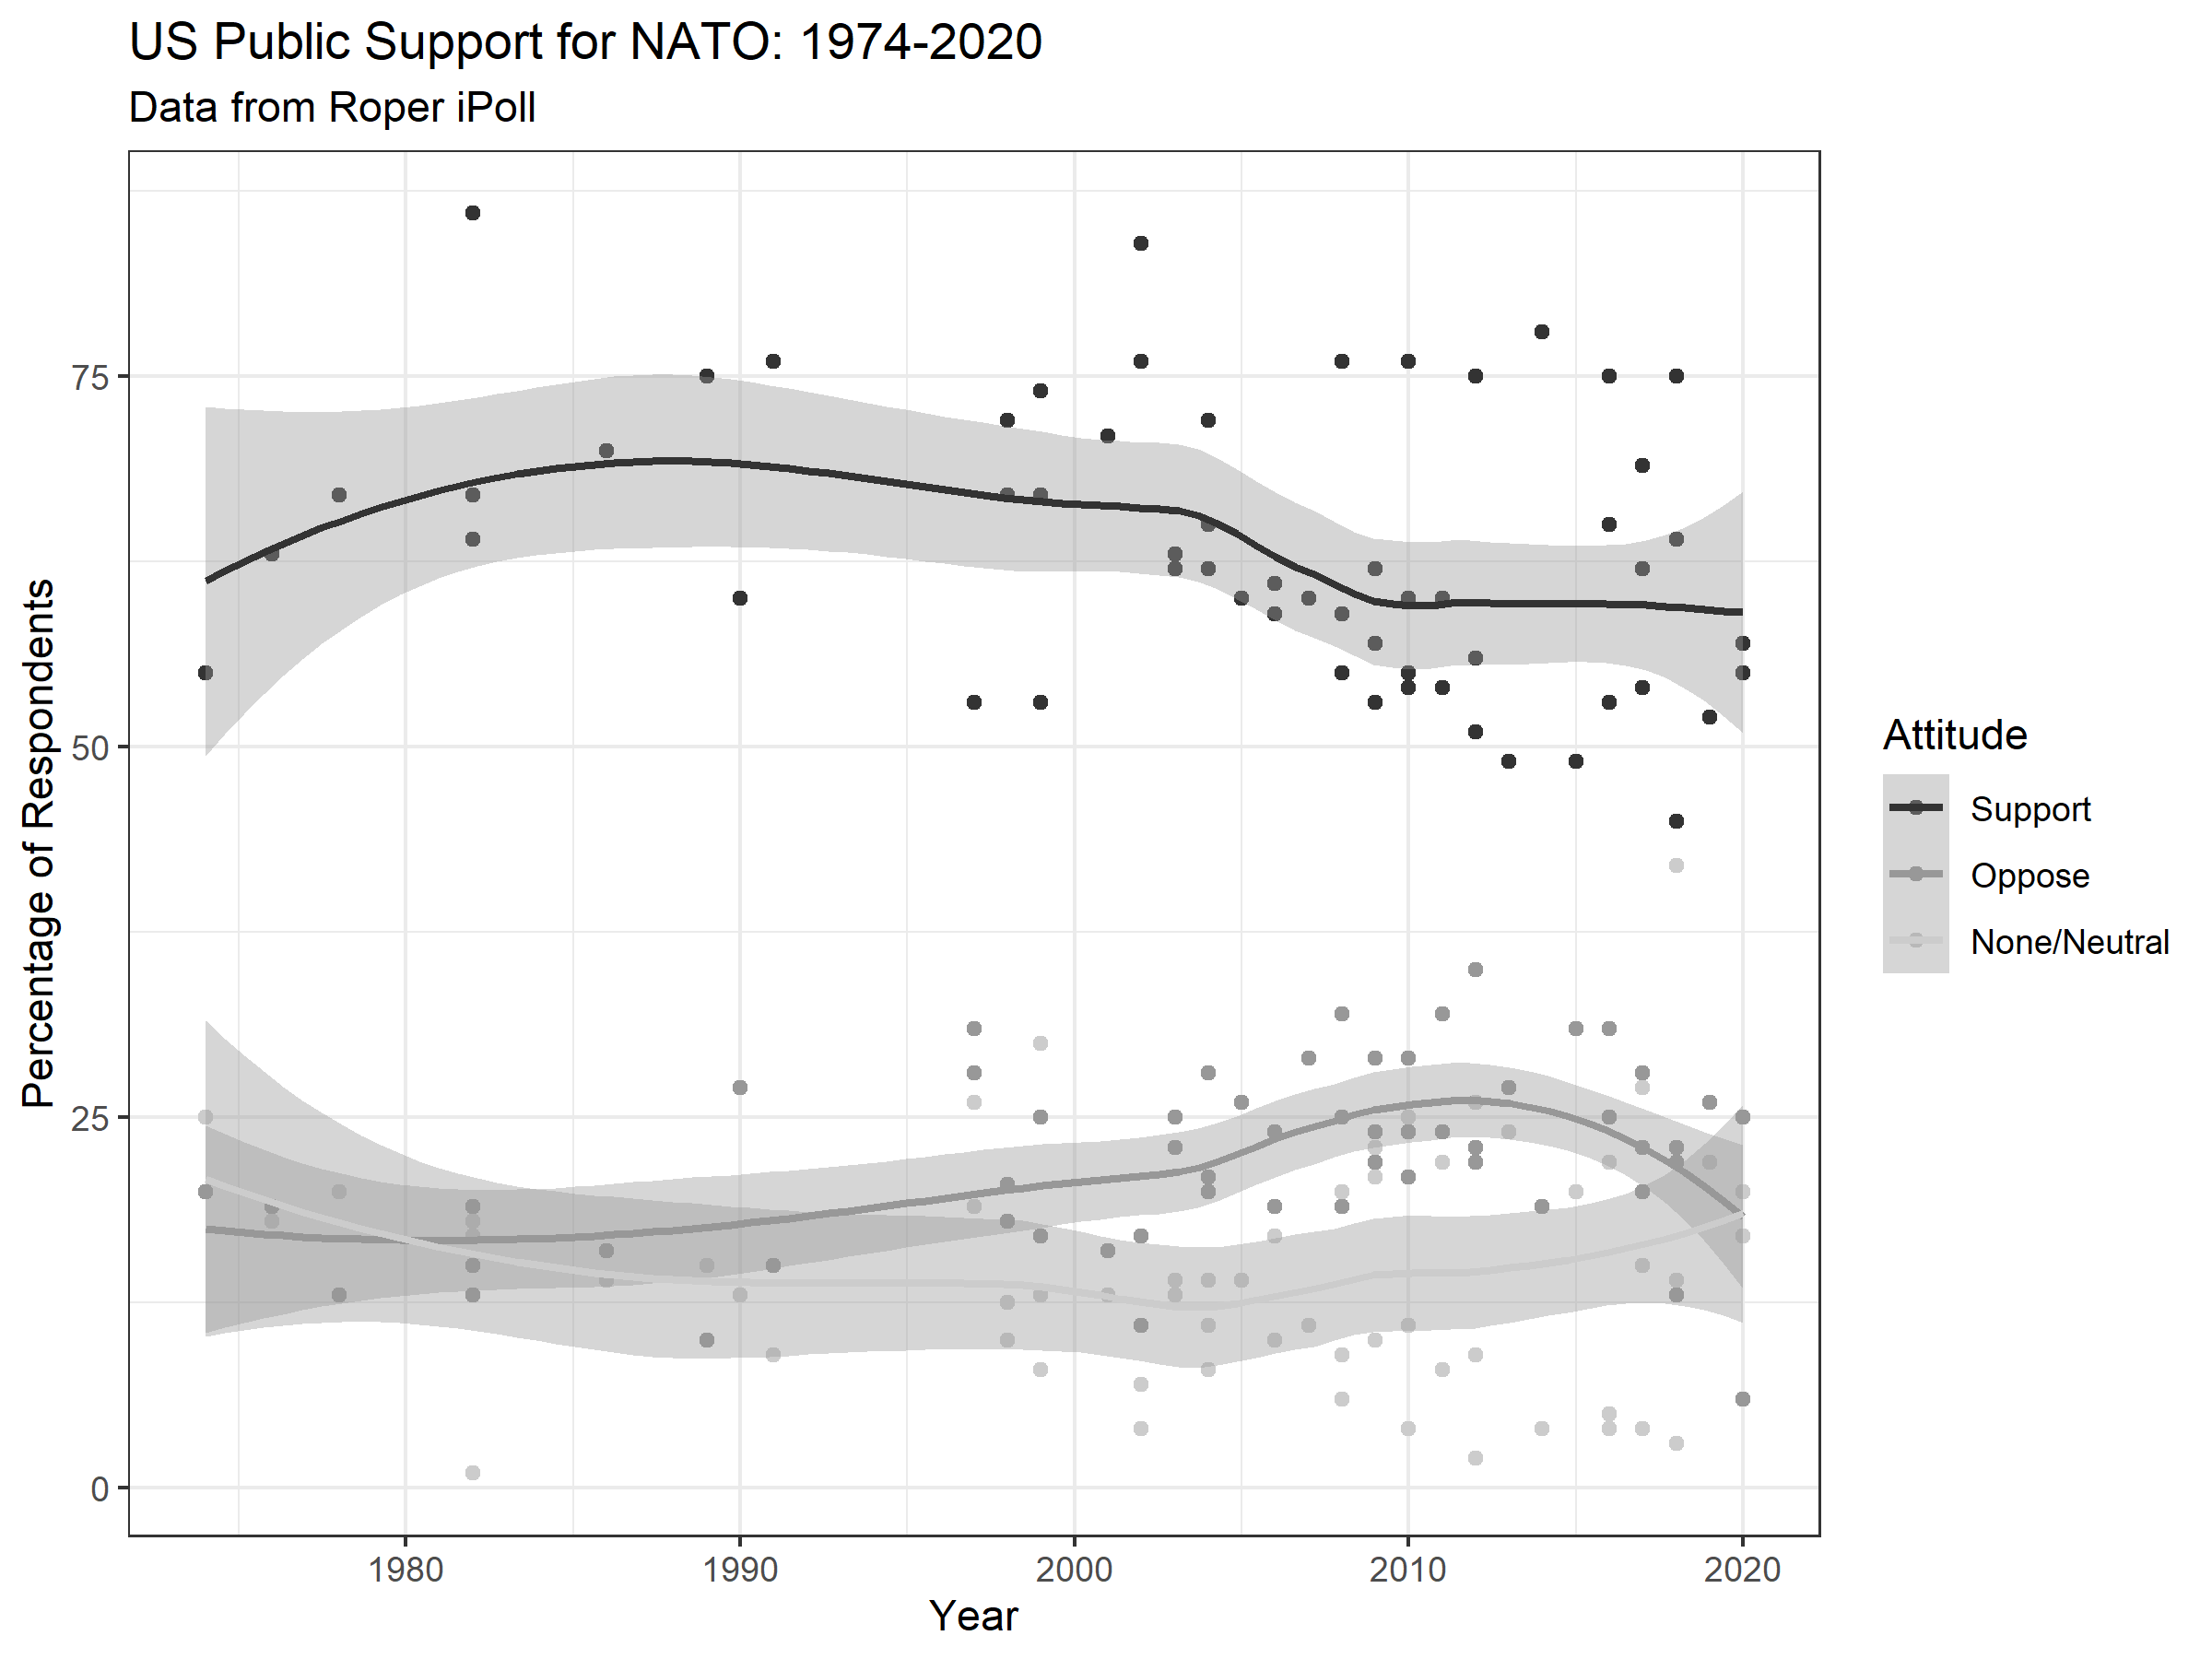
\includegraphics[width=0.95\textwidth]{../figures/nato-op-time.png}
	\caption{US public support for NATO from 1974 to 2020. Each point marks a unique poll, and colors differentiate the percentages of respondents that expressed support, opposition or neutral/no opinion of NATO. Loess lines estimate the average support for each group in every year. Topline data from the Roper Center's iPoll database.}
	\label{fig:nato-op-time}
\end{figure}



Observed alliance attitudes are subject to a common puzzle in public opinion on foreign policy--- who leads whom? 
Put differently, it is unclear if public attitudes towards alliances a top-down result of elite cues or do elite cues reflect existing attitudes. 
Both leading and pandering are plausible models. 


Evidence on whether elites pander to or lead public opinion is divided.
Some suggest that elite pandering is rare. 
\citet{Canes-Wrone2006} finds that Presidents rarely pander to the public unless they already agree with public preferences.
\citet{Kreps2010} notes that public disapproval did not constrain participation in NATO's International Security Assistance Force in Afghanistan. 
Moreover, foreign policy is a secondary concern for many voters, so elite foreign policy views and rhetoric can diverge from public attitudes with few political repercussions \citep{BusbyMonten2012}. 


Other studies suggest that elites match their rhetoric and policy stances to public opinion. 
\citet{Barberaetal2019} use social media data to show that legislators are more likely to follow than lead public opinion on issues. 
Similarly, \citet{HagerHilbig2020} find that exposure to public opinion research moves speech and policy positions by German politicians closer to majority opinion. 
\citet{GuisingerSaunders2017} note than for issues with low partisan polarization, information effects can dominate public opinion, though elite cues matter more for polarized issues like cap and trade schemes. 
\citet{Haesebrouck2019} finds little evidence that European elites led their public to support military interventions in Libya and the Islamic State. 
\citet{Bechteletal2015} find that elite cues and frames lead Swiss individuals, especially those with low knowledge, to reinforce their existing attitudes. 
Even military elites shape their recommendations in response to public opinion \citep{LinGreenberg2021}. 



Alliance attitudes are subject to this puzzle or who leads whom. 
On the one hand, limited public information about alliances could give elite cues and framing substantial influence \citep{Druckman2001}. 
On the other, the public opinion towards alliances may depend on individual dispositions and intuitions about international affairs \citep{Herrmannetal2009, KertzerZeitzoff2017}.
\citet{PageShapiro1992} note that public opinion is broadly consistent and rational, and changes in predictable ways in response to information from multiple sources, including elite cues. 

 
While the top-down model asserts that elites lead public opinion, leaders might pander to existing public attitudes.
Under a pandering framework, convergence between elite rhetoric and public opinion reflects elites conforming their support to public opinion, rather than shaping public attitudes. 
If elite rhetoric on alliances panders to relatively fixed opinions, then elite cues will have little impact.


Alliance attitudes are thus part of fundamental debates about public opinion on foreign policy.  
In the following, I unpack when the public opinion towards alliances is plastic or rigid in the face of elite cues.  
First, I explain how elite cues can influence alliance attitudes. 


\subsection{Elite Cues} 
% Framing/elite leading
% Debate over leading/pandering

Elite cues are a plausible explanation of alliance attitudes. 
In this model, elite portrayals of alliances bolster or undermine public support for alliance commitments as the public follows trusted elites in forming their opinion.
Thus, public opinion towards alliances is endogenous to elite views \citep{Druckman2014}.


If elite cues are the most important factor, public opinion towards alliances is largely a top-down phenomenon.
There is also substantial evidence that elites influence public foreign policy attitudes \citep{BaumPotter2008}. 
The media often convey elite frames and social media may further amplify elite influence \citep{BaumPotter2019}.   


Furthermore, information shortcomings make individuals more responsive to elite framing and cues \citep{Druckman2001, Peterson2017}.  
The public has limited information about foreign policy relative to domestic issues, and alliance politics are not usually salient even within foreign policy. 
Therefore, elite support or opposition could have a profound influence on alliance attitudes as individuals rely on knowledgeable and trusted elites. 


% cue-giver matters
There are multiple potential elite leaders in alliance attitudes. 
Elected officials, diplomats and military leaders are all potentially influential elites in alliance politics. 
Cues from military leaders can shape public opinion about the use of force \citep{Golbyetal2018}, so military endorsements may be especially influential. 
Public perceptions that military leaders and diplomats are well-informed about alliances will likely increase their influence. 


% highlight partisanship 
Partisanship has an important role in elite influence.
With extensive partisan polarization, individuals discount messages from out-partisan elites. 
Conversely, trust increases the influence of messages from co-partisan elites \citep{Druckmanetal2013}. 
According to the elite cues model, support for alliances by trusted elites should increase individual support for alliances, and opposition will reduce public support.  
Unified elite cues would be especially influential, as they increase support in both parties.
For example, \citet{Berinsky2007} finds that unified elite support for war also increases public support. 


% transition paragraph: scope of influence
Elite cues offer a straightforward explanation of alliance attitudes, and elites almost certainly have substantial sway over alliance attitudes.
Even information about alliance characteristics likely reaches the public through elite sources. 
The scope of elite influence may vary, however.
Individual foreign policy dispositions and partisanship could modify the impact of elite cues. 


\subsection{Individual Concerns}
% Kertzer stuff- bottom up


% Overview para
Foreign policy dispositions and partisanship shape perceptions of the costs, benefits and value of international cooperation. 
Therefore, they have two potential consequences. 
First, they could establish individuals' baseline alliance support, or willingness to back alliances in general. 
Second, individual concerns could make individuals more or less responsive to elite cues and particular alliance characteristics. 


% foreign policy disposition
Many individuals have stable intuitions about the best way to approach international politics. 
Militant assertiveness and internationalism are two key foreign policy dispositions \citep{Herrmannetal1999}.  
These principles shape how individuals respond to foreign policy decisions, such as backing down from promises of military intervention \citep{KertzerBrutger2016}. 


% internationalists more likely
% Define internationalism  
Internationalism reflects an inclination to work with other countries and contribute to international institutions. 
Internationalist respondents generally support American engagement in foreign affairs and will likely favor alliance commitments. 
Conversely, isolationist respondents are more skeptical of international institutions and cooperation \citep{Kertzer2013}. 
Isolationists distrust foreign involvement and emphasize domestic affairs. 
As a result, isolationists should be generally skeptical of alliances, and especially opposed to alliances with high financial cost, unconditional support promises or deep cooperation. 


% militant assertiveness 
Militant assertiveness likely increases support for alliances. 
Hawkish individuals are more willing to use force to address international problems. 
Although alliances are a cooperative institution, they also aggregate military capability \citep{FordhamPoast2014}, and call on members to support one another in war.
Hawks will likely support capability aggregation through alliance commitments and be willing to bear the risks of foreign wars.  
Dovish individuals are skeptical of using military force in general, so they will be less likely to support military alliances. 


%% material interests- trade/investment
%In addition to foreign policy dispositions, individuals may have material interests in backing international alliances.
%Military alliances promote economic ties between members, including trade \citep{Gowa1995, LongLeeds2006}, foreign investment \citep{LiVashchilko2010} and currency pegs \citep{Li2003}. 
%Just as individuals who benefit from international commerce back trade liberalization \citep{RhoTomz2017}, individuals with internationally-oriented occupations and economic interests could support alliances that bolster international commerce or protect trade partners. 
%On the other hand, individuals who lose out from lost trade protection under an alliance \citep{WolfordKim2017} are more likely to oppose alliances.


% partisanship 
Partisanship is connected to foreign policy dispositions and material interests. 
Conservatives in the United States have a longstanding history of isolationist sentiment, for instance \citep{Kupchan2020}.
As a result, they are usually more skeptical of international engagements like alliances. 
Republicans also tend to be more hawkish as well \citep{Gries2014}. 
Partisanship may thus encompass the key foreign policy dispositions and dominate individual alliance attitudes. 


Party identification also connects elite cues and individual concerns, as it may amplify the influence of some elite cues and diminish the impact of others.
Individuals look to cues from trusted elites, often from their party. 
Given partisanship's reflection of foreign policy dispositions and connections to elite cues, it may have substantial influence on alliance attitudes. 


% partisanship puzzle
At the same time, because partisanship and foreign policy dispositions are correlated, disentangling them is essential. 
In particular, any analysis must establish whether partisan differences in alliance attitudes are the result of party affiliation or foreign policy attitudes that are correlated with partisanship. 
To do this, I will compare the alliance attitudes of Democrats and Republicans with similar foreign policy dispositions. 
If Republicans and Democrats with similar foreign policy dispositions hold distinct alliance attitudes, this implies that partisanship has some influence. 


\subsection{Leading, Pandering and Individual Concerns}


% limits 
Understanding who leads and who follows in alliance attitudes requires careful attention to elite cues, partisanship and foreign policy dispositions. 
Estimating whether elite cues generally increase public support for alliances cannot differentiate between pandering and leading. 
This is especially true because partisanship is correlated with foreign policy dispositions like isolationism and militant assertiveness that shape baseline alliance attitudes. 
Perhaps Republican leaders' opposition to alliances does not decrease Republican support for alliances, it simply reflects conservative isolationism, for example. 


% how distinguished
To assess who leads and who follows, I leverage the confluence of partisanship and foreign policy dispositions.
I examine how co-partisan elite cues impact Democrats and Republicans with different initial dispositions towards alliances.
Initial alliance dispositions from militant assertiveness and isolationism may make individuals more or less responsive to elite cues. 


% explain 
If cues pander, isolationists will be less responsive to cues from co-partisan elites.
But if elites lead public opinion, co-partisan elite support will increase support for alliance participation even among isolationists. 
If elite support increases alliance support among isolationists, elites can lead alliance attitudes. 
Similarly, hawkish individuals might discount elite cues if they back most alliances and elites cues pander. 
But if elite opposition reduces support among hawkish individuals who are otherwise strong alliance supporters, elite cues lead public opinion towards alliances. 


% no a priori about different combinations
The salience of isolationism and hawkishness in alliance attitudes creates four relevant foreign policy dispositions within each party. 
Individuals may be isolationist and hawkish, internationalist and hawkish, isolationist and dovish, or internationalist and dovish.
While some existing research does not divide isolationists into hawks and doves and distinguishes between cooperative and militant internationalists \citep{Kertzeretal2014}, I divide isolationists as well to assess the net impact of competing dispositions.\footnote{To streamline discussion across the four categories, I do not use the terms cooperative and militant internationalism in the manuscript, though the concepts are equivalent.}  
I do not have strong priors about the relative strength of hawkishness and isolationism, however.
One effect could dominate the other, the two factors could offset, or they could interact in unexpected ways.


% dividing partisans
Dividing respondents into these groups provides clear leverage over who holds plastic or rigid alliance attitudes. 
Taking this approach allows me to identify who follows elite cues. 
While most of the results focus on elite cues, I also consider alliance characteristics. 




\subsection{Alliance Characteristics}
% some alliances are more attractive than others
% look to other results- democ, strength, etc. 
% economic interests


Military alliances take many forms, as states negotiate distinct treaties with diverse partners.
Allied capability, shared interests, and the nature of the alliance obligations are all plausible determinants of alliance attitudes.   
Limited public information on foreign policy issues may constrain the impact of alliance characteristics, however. 
Most information about alliance characteristics likely comes from elites, attached to cues in some way \citep{BaumPotter2008}. 


% Capability
Allied capability is the first major alliance characteristic.
Greater allied capability should generally increase the appeal of an alliance. 
All else equal, alliances with militarily capable states are more valuable \citep{Johnsonetal2015}. 
Inasmuch as the public understands that allies with substantial military capability have greater capacity to deter and fight, they will back alliances with more capable states. 


% Shared interests
Perceptions of shared interests with allies are another salient alliance characteristic. 
Common threat, economic ties, recent military operations democratic political institutions are all observable indicators of common interests. 
The public may only be willing to hazard the costs of intervention under serious threat. 
If individuals do not believe that the alliance addresses a security threat, they will be less likely to support protecting foreign states.
Protecting trade ties often motivates asymmetric alliances between large and small states \citep{Fordham2010}. 
As individuals value foreign trade and investment and see it as an indicator of common interests, they will approve of alliance commitments with trade partners. 
If the United States and a potential alliance partner or current ally recently participated in a common military operation, the public could believe that they share common concerns and interests. 
Recent military operations would also suggest that the other state will bear substantial costs to support the United States.\footnote{Some states may have participated in wartime coalitions to encourage closer ties with the United States \citep{GannonKent2020}.}


% Democracy 
Democratic citizens may also prefer alliances with other democracies. 
At a minimum, the democratic public rarely supports military strikes against other democracies \citep{TomzWeeks2013}. 
Individuals may believe that democracies should cooperate because they share common concerns and values. 
Shared values are a plausible justification of alliance participation \citep{Chuetal2021}. 
Domestic political regimes thus offer a simple heuristic for a trustworthy and valuable alliance partner. 


% Alliance treaty design 
In addition to shared interests, alliance obligations may shape public support for alliances, especially alliance formation. 
There is immense variation in alliance treaty content \citep{Leedsetal2002}.
Potential alliance members must agree on whether they are willing to offer military support, conditions on that support, and how they will contribute to deterrence and/or war fighting \citep{Poast2019a}. 
These issues are reflected in alliance treaties, which stipulate military intervention, conditions on allied support, defense cooperation, and issue linkages, all of which could impact alliance attitudes. 


% conditionality, depth and issue linkages
If the public fears entrapment in foreign conflicts or reckless allies, they will prefer alliances with conditional obligations.
Most U.S. alliances restrict promises of intervention to attacks on allies and conflicts in specific regions. 
Other alliances supplement the core promises of military support with peacetime defense cooperation \citep{Morrow1994, LeedsAnac2005} to coordinate policies and establish credible commitments.
Almost half of all military alliances have some defense cooperation \citep{Leedsetal2002}, and many U.S. alliances include formal organizations, bases, and military aid. 
The public may prefer more arms-length commitments, or back strong ties with allies. 
Last, formal and informal issue linkages often facilitate agreement and support credible alliance commitments \citep{Poast2012, Poast2013}. 
Perceptions that an alliance brings further trade or foreign policy concessions could increase public approval, as the public perceives tangible alliance benefits.  



% financial costs
In addition to formal treaty obligations, military alliances increase U.S. defense spending \citep{AlleyFuhrmann2021}. 
While the public may accept the costs of alliances, alliance skeptics often highlight the financial costs of alliance commitments \citep{Posen2014}. 
Military spending on alliances has opportunity costs, as funds spent on the military are not used for other goods. 
Thus, more expensive commitments command less public support, especially among isolationists. 

 
% how to think about characteristics
These alliance characteristics primarily serve as controls. 
Whether given characteristics are bundled with elite cues, providing additional information about the alliance ensures the any impact of elite cues is not driven by inferred alliance characteristics.
The potential impact of different alliance characteristics is also interesting in its own right. 


% formation vs maintenance
Before discussing the research design, there are two important considerations. 
First, alliance formation and maintenance are distinct processes \citep{Snyder1997}. 
Forming a new alliance and upholding an existing commitment are subject to different considerations.
Therefore, I consider alliance formation and maintenance in separate survey experiments to assess whether the public views making a new alliance commitment and upholding an existing treaty differently. 


%-------------------------------------
% % cut over time for the moment
%% explanation over time
%The elite cues model can predict changes in alliance attitudes over time. 
%In this framework, shifting public attitudes reflect new elite cues. 
%Conversely, stable public opinion would indicate consistent elite views. 
%
%
%% change over time: generations
%Individual concerns could explain changes in public support for alliances over time through generational shifts. 
%As the experiences of each generation mold their foreign policy dispositions, public opinion of alliances will slowly shift over time. 
%Such gradual shifts in public opinion towards alliance commitments are perhaps consistent with some of the observed data in \autoref{fig:nato-op-time}. 
%
%
%% shared interests and cap as key explanations of changes over time. 
%Indicators of shared interests and changes in allied capability could explain temporal variation in alliance attitudes. 
%Threat perceptions and recent military operations are both salient contextual factors. 
%If public perceptions of common interests wane, support for alliances will fall. 
%For example, reduced allied capability could create beliefs that partners are not pulling their weight or contributing enough capability. 
%Democratic backsliding might also lead the public to question whether allies share U.S. interests and values. 
%
%% obligations are less dynamic
%Alliance obligations are less likely to explain changes in public opinion over time than individual dispositions or contextual factors like threat, trade and allied democracy. 
%Fixed treaty obligation cannot explain variation in alliance attitudes over time. 
%Treaty obligations could affect public support for treaty formation, however. 
%--------------------------------------------



% long-run cycles
Second, feedback between elite cues and public opinion is plausible in the long run. 
It is possible that public opinion shapes elite cues, which in turn alter public opinion. 
For example, elites could respond to growing public opposition to an alliance by pandering and adopting more skeptical rhetoric. 
Elites could also attempt to lead public opinion and restore alliance support, however.
Such feedback takes time, and would be most obvious in the context of longstanding alliances.
If such a cycle exists, elite cues must influence alliance attitudes.
This analysis can therefore establish part of a potential feedback cycle. 
I now describe how I assess the role of elite cues in alliance attitudes. 



\section{Experimental Design}


% justify conjoint: 
I use two conjoint survey experiments to unpack the sources of public support for forming and maintaining alliances in the United States. 
Observed alliances bundle elite support and characteristics like threat and treaty obligations, each of which is a potential experimental treatment.  
Conjoint experiments allow researchers to decompose composite phenomena to estimate and compare the impact of multidimensional treatments \citep{Hainmuelleretal2014}. 
For example, \citet{HainmuellerHopkins2015} use a conjoint experiment to identify what types of immigrants Americans favor. 
\citet{BechtelScheve2013} assess how institutional design affects public approval for climate cooperation agreements with a conjoint experiment in four countries. 


% describe rating tasks
Both conjoint experiments ask individuals whether they support participation in a defensive military alliance that has a randomly generated profile of alliance characteristics and elite cues. 
In the alliance formation experiment, I ask respondents to assess five hypothetical new alliances. 
In the alliance maintenance experiment, respondents rate five hypothetical existing alliance commitments.


Before presenting the alliance rating tasks, I measure key respondent characteristics, especially partisanship and foreign policy disposition.  
These measures provide the basis of the subgroup analyses examining how individual concerns shape alliance attitudes. 
The subgroup analyses assess whether baseline support for alliance participation differs across groups and how the impact of elite cues and alliance characteristics varies.


After measuring key individual factors, I present respondents with a table of information about a hypothetical alliance with a randomly generated profile of elite cues and characteristics.
Once respondents read the table, I then ask them to rate the alliance on a scale from 0 to 100 and express approval of alliance formation or maintenance with a yes/no question. 
I will then present four more randomly generated alliance profiles, so each respondent rates five hypothetical alliances in a single-profile conjoint design.\footnote{A two profile design would ask respondents to choose between two alliances, each with a random set of characteristics.} 


% Add a table with conjoint attributes. 
Each alliance partner profile is randomly generated from the attributes in \autoref{tab:conjoint-vars}.
Every attribute has multiple potential values and I produce the full alliance profile by randomly selecting one value from each attribute. 
I chose the set of attributes and values to capture theoretically interesting alliance characteristics and generate plausible profiles.\footnote{There are no restrictions on value combinations in the alliance profiles. I employ this uniform randomization because all of these alliance profiles are plausible. This also has the advantage of generating substantial variance in elite cues.} % De la cuesta et al discussion here as needed
I randomize the order of the attributes in the table at the respondent level, so the order is the same for each respondent. 
Drawing alliance profiles at random and providing multiple rating tasks in a conjoint experiment makes estimating the average marginal component effect (AMCE) for each alliance attribute straightforward \citep{Hainmuelleretal2014}. 


\begin{table}
\begin{adjustbox}{width = .99\textwidth}
\begin{tabular}{lc} 
\hline \\ 
\textbf{Attributes} & \textbf{Values} \\
\hline \\ 
Republican Senators & Support an alliance with this country. \\
                    & Oppose an alliance with this country. \\ 
                    
Democratic Senators & Support an alliance with this country. \\
                    & Oppose an alliance with this country. \\ 
                    
The Joint Chiefs of Staff & Support an alliance with this country. \\
                    & Oppose an alliance with this country. \\ 
                    
The Secretary of State & Supports an alliance with this country. \\
                    & Opposes an alliance with this country. \\ 
                    
Trade Ties          & The United States has minimal trade ties with this country. \\
                    & The United States has modest trade ties with this country. \\
                    & The United states has extensive trade ties with this country. \\ 
% modified from Tomz and Weeks 2013 APSR: https://web.stanford.edu/~tomz/pubs/TomzWeeks-2013-11-Appendix.pdf 
Partner Political Regime    & This country is not a democracy, and shows no sign of becoming a democracy. \\
                    & This country is a democracy, but shows signs that it may not remain a democracy. \\ % democ backsliding
                    & This country is a democracy, and shows every sign that it will remain a democracy. \\
                    
Partner Military Capability & 10,000 soldiers and spends 1\% of their GDP on the military. \\ % low
                    & 80,000 soldiers and spends 2\% of their GDP on the military. \\ % moderate
                    & 250,000 soldiers and spends 3\% of their GDP on the military. \\ % high 
                    
Shared Threat       & The United States and this country face minimal common threats. \\ 
                    & The United States and this country face modest common threats. \\
                    & The United States and this country face serious common threats. \\
                    
Recent Military Cooperation  & This country has not participated in recent U.S. military operations. \\ 
                    & This country recently supported U.S. airstrikes against terrorists. \\
                    & This country recently supported U.S. counterinsurgency operations. \\
                    & This country recently fought with the United States in a war. \\
                    
Financial Cost      & This alliance requires \$5 billion in annual U.S. defense spending.  \\ 
                    & This alliance requires \$10 billion in annual U.S. defense spending.  \\ 
                    & This alliance requires \$15 billion in annual U.S. defense spending.  \\ 
                    
Conditions on Support  & The alliance treaty promises military support in any conflict. \\ 
                    & The alliance treaty promises military support only if this country did not provoke the conflict. \\ 
                    & The alliance treaty promises military support only if the conflict takes place in this country's region. \\
                    
Defense Cooperation & None. \\ 
                    & The alliance treaty provides basing rights for U.S. troops. \\
                    & The alliance treaty includes a shared military command. \\
                    & The alliance treaty includes an international organization to coordinate defense policies.  \\ 
% Issue linkages                    
Related Cooperation & None. \\
                    & The alliance is linked to greater trade and investment with the United States. \\ 
                    & The alliance is linked to greater support for the United States in the United Nations. \\ 
                    
Region              & Europe. \\ 
                    & Africa. \\
                    & The Middle East. \\ 
                    & Asia. \\   
                    & The Americas. \\ 
                                                                            
\hline \\
\end{tabular}
\end{adjustbox}
\caption{Table of alliance attributes in conjoint experiment profiles. I use the same set of attributes as treatments in the alliance formation and maintenance experiments.} 
\label{tab:conjoint-vars}
\end{table}


% summarize table
As \autoref{tab:conjoint-vars} shows, I include many salient alliance attributes.
Support or opposition from Republican and Democratic Senators, the Joint Chiefs of Staff, and the Secretary of State provide elite cues from elected officials, military leaders and diplomats. 
Other attributes cover key alliance characteristics such as trade ties, regime type, shared threat, military capability, conditions on support, defense cooperation, and issue linkages.
The regime type indicator includes nondemocracy, fragile democracy, and consolidated democracy to examine whether democratic backsliding affects public attitudes towards alliances. 
The financial cost values reflect the most conservative relationship between an alliance commitment and U.S. military spending from \citet{AlleyFuhrmann2021}. 
I also randomize the region of the hypothetical alliance partner to mitigate confounding.  


% Justify number of attributes
Each hypothetical alliance has fourteen attributes.
This ensures that attributes do not mask one another, but also that respondents are not overwhelmed and reduce the effort they put into assessing the full profile.
Studies of satisficing in conjoint experiments suggest that including fourteen attributes in a profile is unlikely to reduce data quality \citep{Bansaketal2019}. 
Furthermore, there is little evidence of satisficing when respondents are asked to rate or compare five profiles \citep{Bansaketal2018}, as is the case in this study.\footnote{I find little difference in treatment effects across rating tasks, which suggests that satisficing is not a major concern.} 


To analyze the results, I first estimate unconditional average marginal component effects.\footnote{In the appendix, I consider an alternative distributions of alliance profiles for this analysis, using the model-based population AMCE method of \citet{delaCuestaetal2021}.}
After that, I estimate interactions between the conjoint treatments and individual considerations.
In particular, I test whether partisanship and foreign policy dispositions modify the impact of elite cues and alliance characteristics. 
I undertake these subgroup analysis by examining the marginal means of support across different groups and employing omnibus F-tests to assess aggregate differences \citep{Leeperetal2020}. 
Marginal means estimate support for a particular choice in a given category, averaging over all other experimental treatments. 



\subsection{Sample and Individual Measures}


There are two experiments--- one for alliance formation and another for maintenance. 
Each nationally representative sample contains 1500 U.S. respondents, recruited through Lucid Theorem.
These results will be under powered for very small effects, but have enough power to pick up most large differences and interactions. 


For each respondent, I measured key individual correlates of alliance attitudes, especially partisan affiliation.\footnote{I classified independent ``leaners'' as Democrats or Republicans, respectively. I coded independents or others that expressed no partisan lean or affiliation as independents.}
I also used standard batteries to measure internationalism and militant assertiveness \citep{Herrmannetal1999, KertzerBrutger2016}.
These measures provide the basis of a series of subgroup analyses. 


Analyzing partisan and foreign policy disposition subgroups in the conjoint experiment requires categorical measures of foreign policy dispositions. 
To divide respondents into isolationists and internationalists, I coded agreement with the most common survey measure as isolationism, and disagreement or a neutral stance as internationalism. 
The hawkishness index is the sum of three questions about the use of force and war. 
Hawkish individuals scored above the midpoint of three on this scale, while doves scored three or lower. 
I then interacted partisanship, hawkishness and isolationism to analyze foreign policy dispositions within partisan groups.


\section{Results} 


In these results, I first present the unconditional average marginal component effect (AMCE) of elite cues and alliance characteristics.
I then consider how a combination of partisan identification, hawkishness and isolationism shapes alliance attitudes. 
I find that elites have substantial power to lead alliance attitudes, but that important subsets of both parties hold more rigid views of alliances. 


\autoref{fig:joint-plot} shows the AMCE of elite cues and alliance characteristics on individual choices in the alliance formation and maintenance experiments.
Given the large number of factors, these figures highlight the most salient AMCE estimates.\footnote{See the choice and rating AMCE figures in the appendix for a full presentation of all the estimates.}


These unconditional estimates are consistent with elite influence on alliance attitudes. 
Elite cues clearly increase public support for alliance formation and maintenance. 
Support from Senators and the Joint Chiefs of Staff is especially influential.
Backing from the Secretary of State has a smaller positive effect. 


\begin{figure}
	\centering
		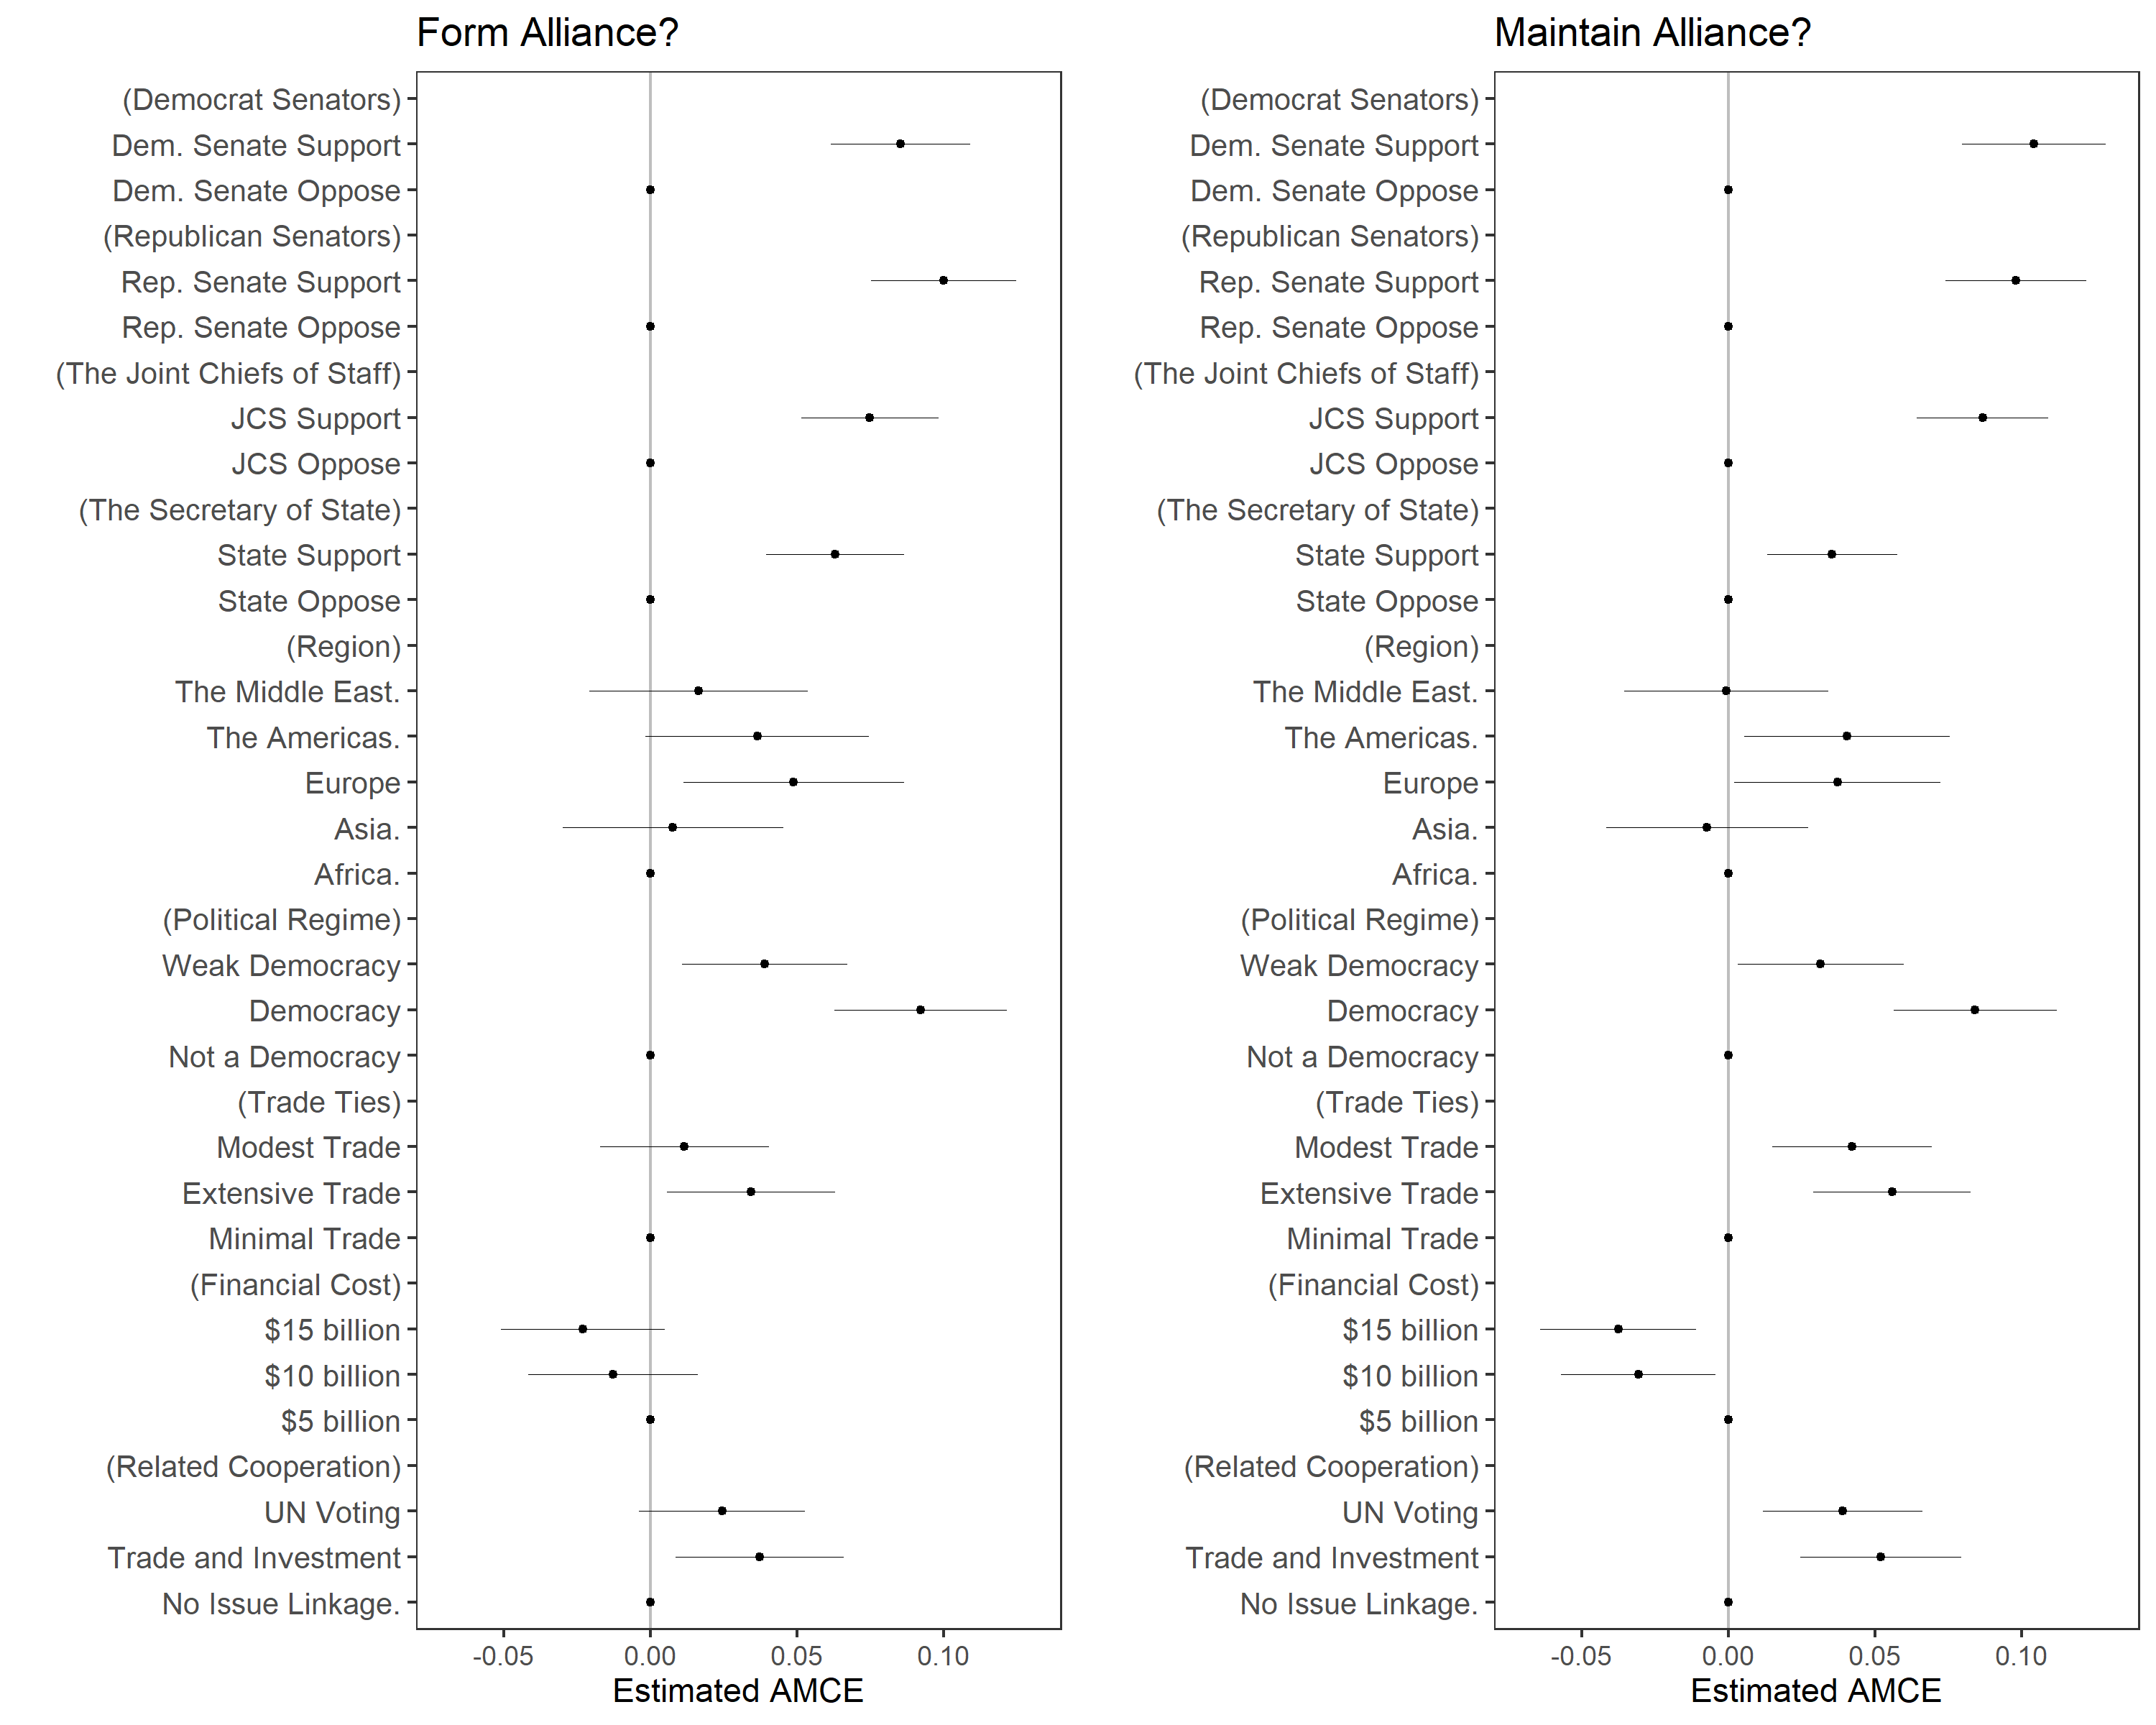
\includegraphics[width=0.95\textwidth]{../figures/joint-amce-plots.png}
	\caption{Average marginal component effect of elite cues and alliance characteristics on public support for forming or maintaining a hypothetical new military alliance. Feature names in parentheses. Components marked with abbreviated labels to make the plot more legible.}
	\label{fig:joint-plot}
\end{figure}


Some alliance characteristics are influential as well. 
Allied regime type is particularly consequential. 
Democracy, especially established democracy, increased support for alliance formation and maintenance.  
Backsliding democracies are marginally more likely than non-democracies to receive public support, but they receive more limited public backing than established democracies.
The magnitude of the established democracy AMCE is comparable to elite cues. 


Issue linkages also encouraged individuals to back alliance formation and maintenance. 
Linkages to trade and investment with the United States were especially influential, relative to an alliance with no such linkages. 
Political issue linkages in the United Nations increased individual support as well, albeit in a more limited way. 
This suggests that issue linkages can facilitate alliance agreements by boosting popular support for new commitments \citep{Poast2012}. 
Last, trade ties and serious common threat encouraged support for alliance maintenance. 
 

Public attitudes towards existing alliances are also sensitive to financial cost.
Relative to the lowest annual cost, annual costs of \$10 billion or more decrease support for upholding an alliance.  
Recent military support could somewhat offset cost concerns, however. 
Allied backing for recent U.S. airstrikes on terrorists increases individual support for an alliance. 


The above results assume that individuals respond in the same way to different cues and alliance characteristics. 
But individual concerns may modify the role of alliance attributes.
The confluence of partisanship and foreign dispositions is especially important for alliance attitudes. 



\subsection{Partisanship, Hawkishness, Isolationism, and Alliance Attitudes}


Leading models predict that individuals will respond primarily to co-partisan or other trusted elites. 
Partisanship is bound up with foreign policy attitudes. 
As as result, it is unclear whether partisan differences in alliance attitudes and responses to elite cues reflect foreign policy dispositions or partisanship. 
In this section, I disentangle support for alliances across respondents with different partisan affiliations and foreign policy dispositions.  


This analysis is essential for establishing whether leaders pander to or lead public opinion. 
If elite cues exert little impact on likely alliance skeptics and strong alliance supporters, they are more likely to follow public opinion. 
On the other hand, if elites cues increase alliance support among likely alliance skeptics and backers alike, this suggests elites can lead public opinion. 


In the following, I present a series of marginal means plots of support for alliance participation within the two major parties.  
I start by focusing on the marginal means of support for different elite cues. 
I then examine how respondents with different partisan affiliations view key alliance characteristics. 


\subsubsection{Elite Cues}

\autoref{fig:party-dispo-form-el} and \autoref{fig:party-dispo-main-el} show the marginal means of support for alliance formation and maintenance across partisans with different foreign policy dispositions under different elite cues.\footnote{See the appendix for details on the distribution of foreign policy dispositions across party identification.} 
Each panel plots the marginal mean of support for every combination of militant assertiveness and internationalism within both parties. 
Both figures show differences in baseline support and responses to the conjoint treatments. 


Alliance attitudes reflect a complex combination of foreign policy dispositions and partisanship. 
The same foreign policy dispositions have distinct implications for alliance attitudes among Republicans and Democrats, so partisanship matters.
At the same time, foreign policy dispositions are responsible for substantial differences in alliance attitudes within parties. 
Therefore, partisanship and foreign policy dispositions both influence alliance attitudes. 


\begin{figure}[htpb]
	\centering
		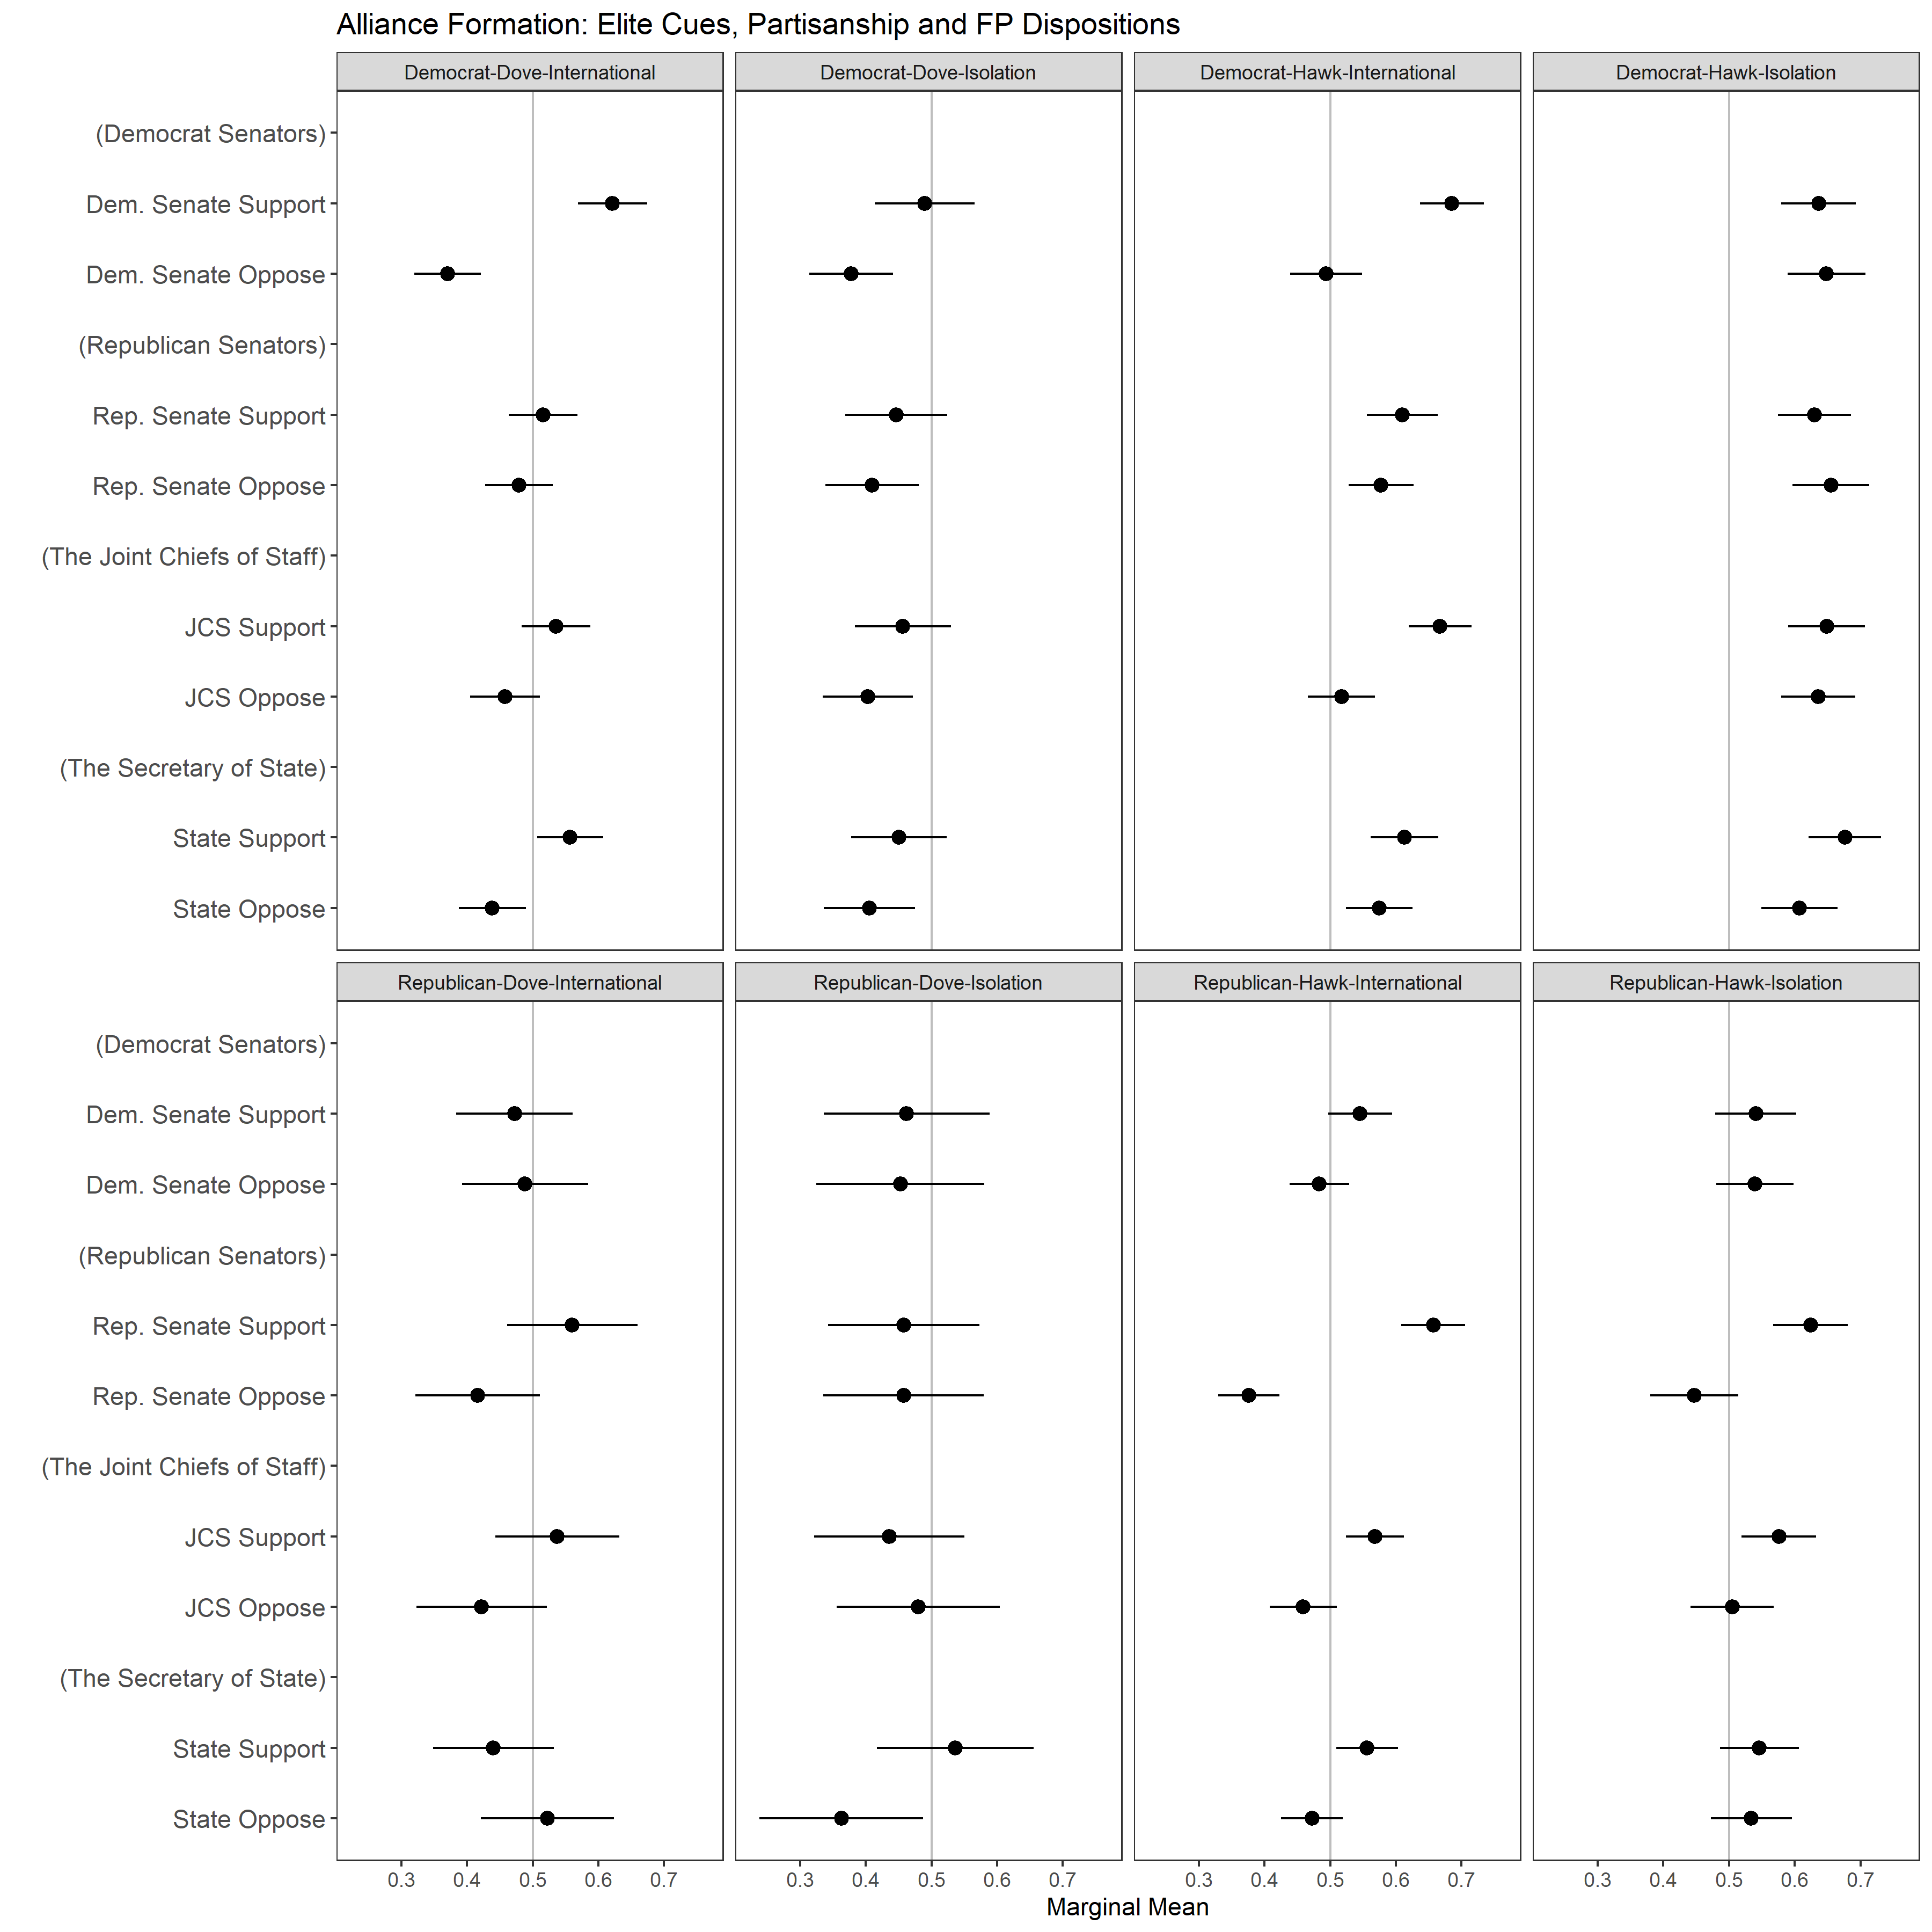
\includegraphics[width=0.95\textwidth]{../figures/party-dispo-form-el.png}
	\caption{Marginal means of support for forming a hypothetical alliances across party identification and foreign policy dispositions under different elite cues. For each group, the estimates mark the marginal mean of support for alliance participation under different alliance treatments. The vertical line highlights a marginal mean of .5, as it is a threshold for majority support. Components marked with abbreviated labels to make the plot more legible. Independents omitted.}
	\label{fig:party-dispo-form-el}
\end{figure}


Among Democrats and Republicans, hawkishness increases general support for alliance participation, as \autoref{fig:party-dispo-form-el} and \autoref{fig:party-dispo-main-el} show. 
This relationship is subject to partisan differences, however, as hawkish Democrats express higher support for alliance formation than hawkish Republicans. 
Hawkish and isolationist Democrats are especially strong supporters of alliance participation. 
Hawkishness also increases support for alliance participation among isolationist Republicans. 
Willingness to support military measures can offset some skepticism of international engagement in alliance attitudes. 


Isolationism alone does not systematically reduce support for alliance participation, as one might expect.
The cumulative impact of skepticism towards international engagement depends on hawkishness. 
Isolationist and dovish individuals are the greatest skeptics of alliance formation and maintenance. 
The combination of isolationism and limited willingness to use force is at the heart of alliance opposition. 
Although few Republicans are doves, they are integral to alliance skepticism in the GOP. 


\begin{figure}
	\centering
		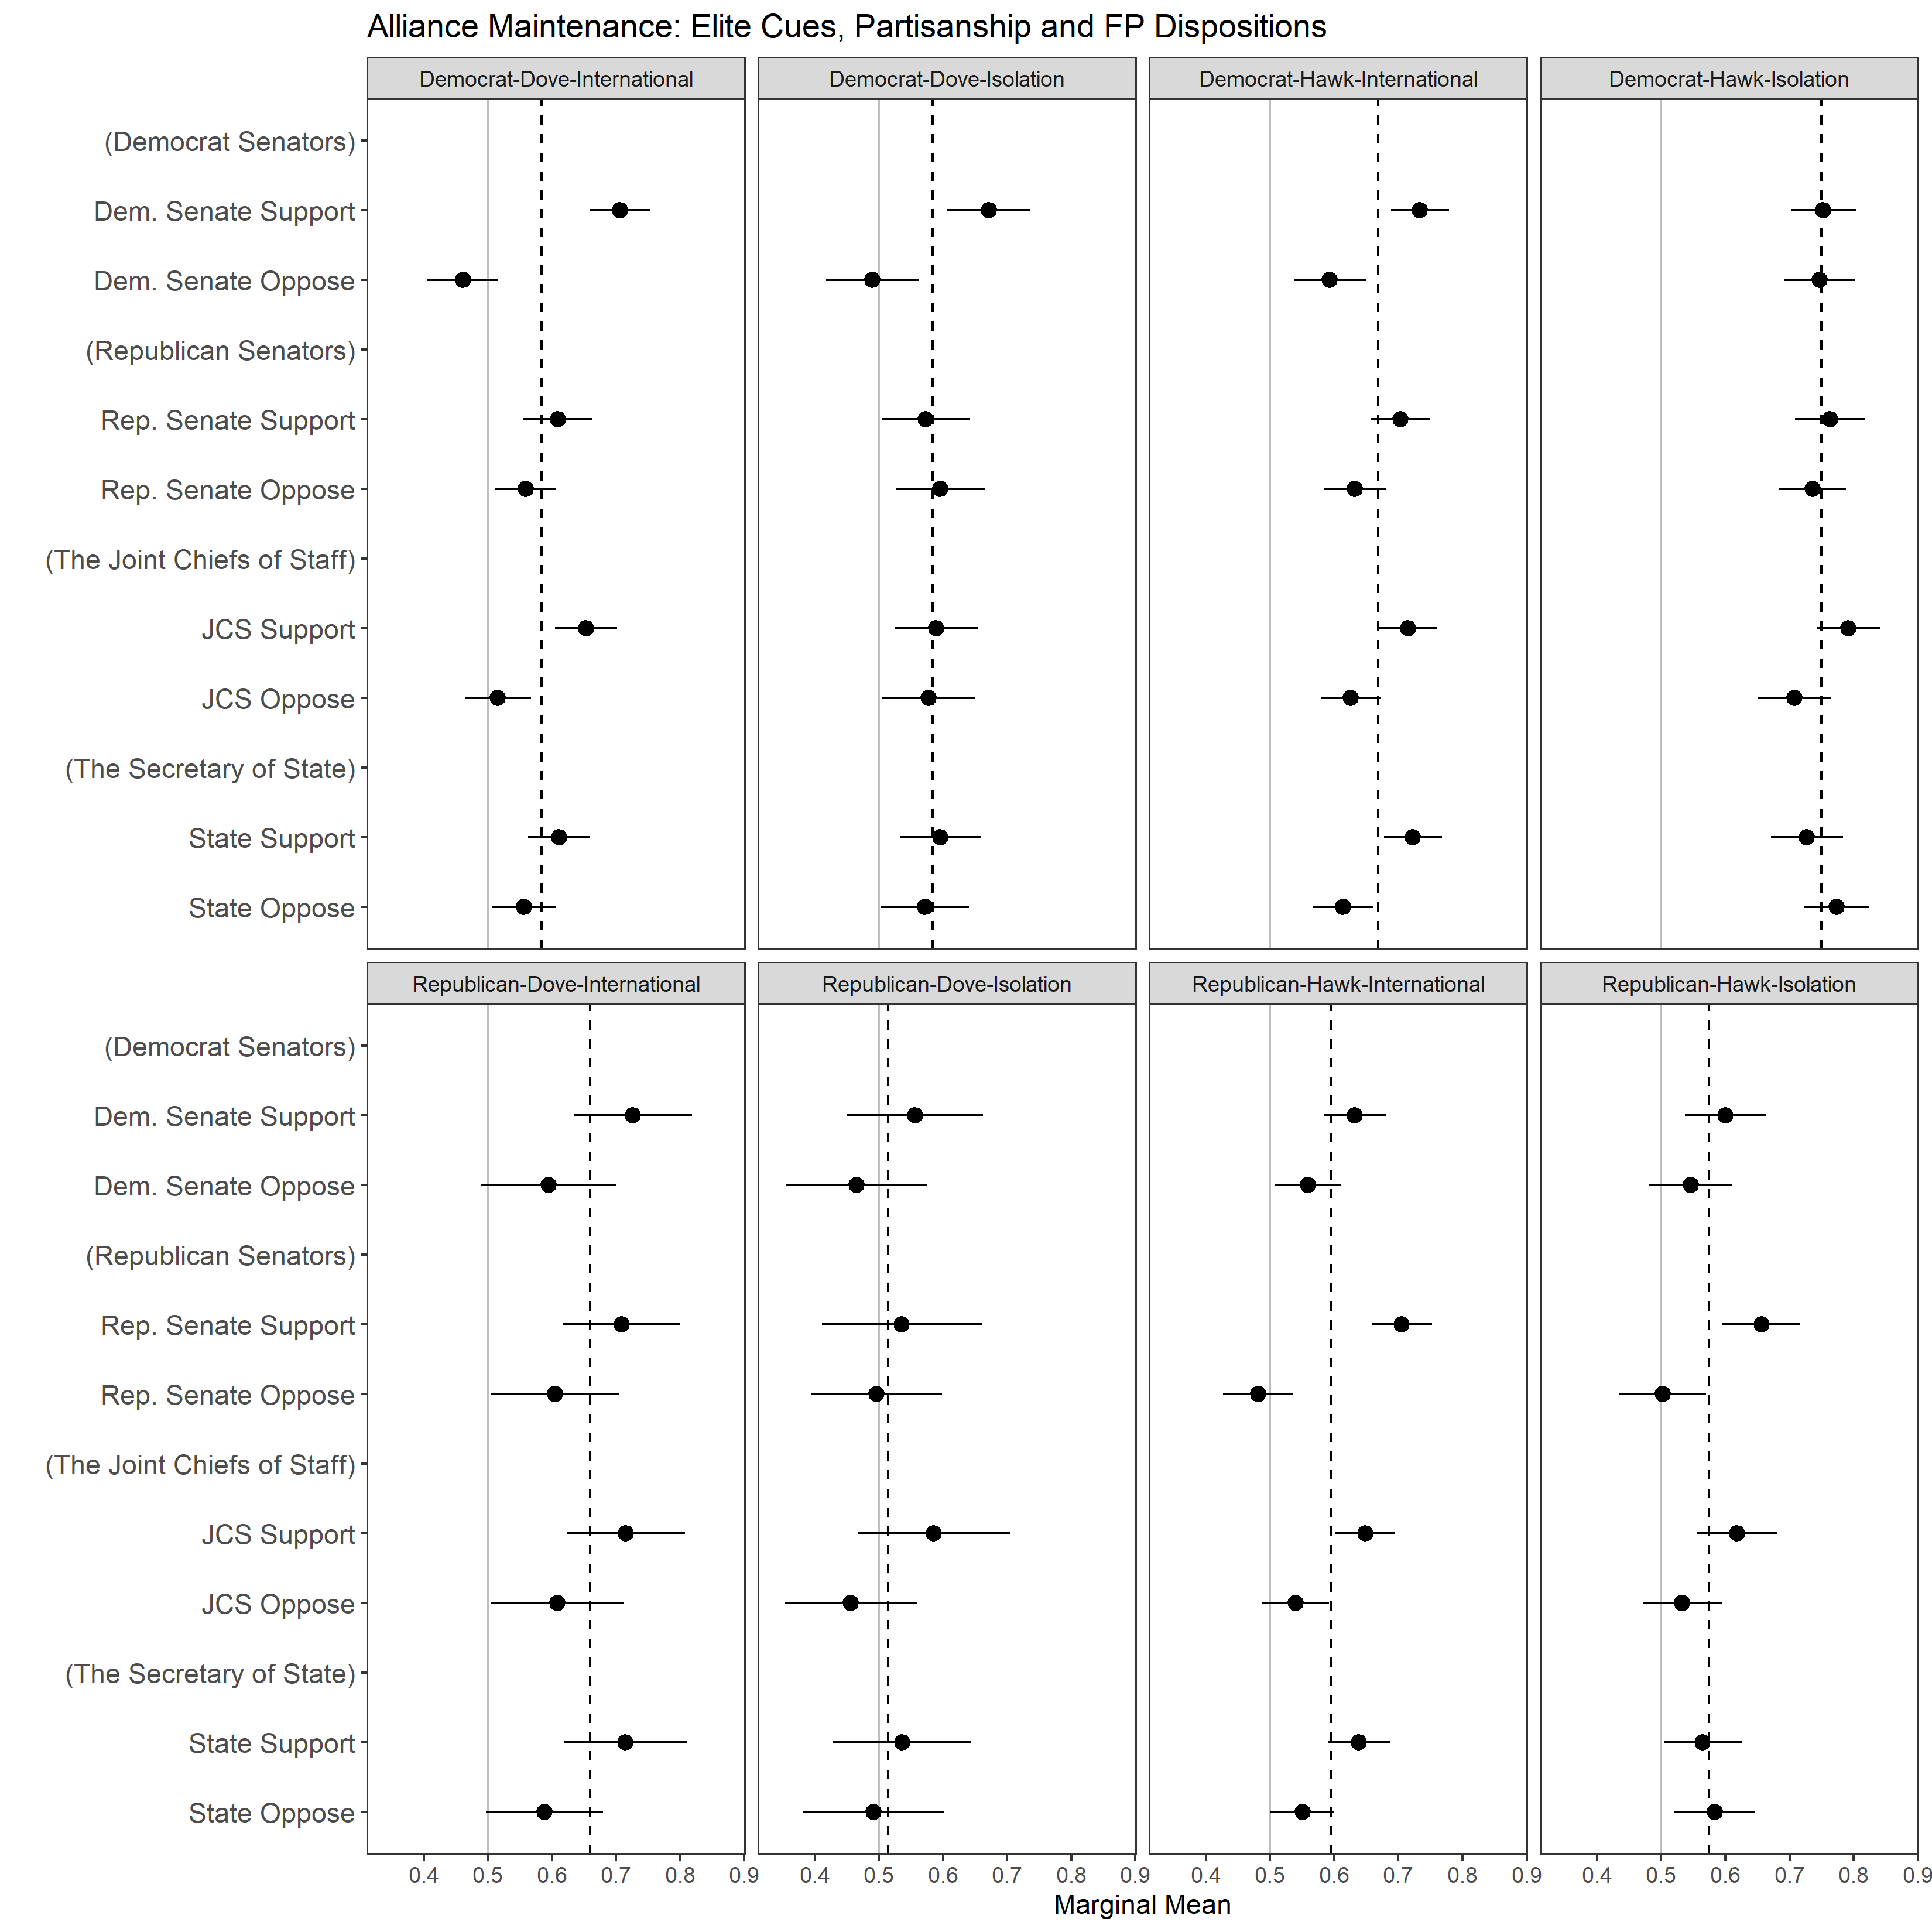
\includegraphics[width=0.95\textwidth]{../figures/party-dispo-main-el.png}
	\caption{Marginal means of support for maintaining a hypothetical alliances across party identification and foreign policy dispositions under different elite cues. For each group, the estimates mark the marginal mean of support for alliance participation under different alliance treatments. Vertical line highlights a marginal mean of .5, as it is a threshold for majority support. Components marked with abbreviated labels to make the plot more legible. Independents omitted.}
	\label{fig:party-dispo-main-el}
\end{figure}


In addition to shifting baseline alliance attitudes, foreign policy dispositions change how individuals respond to elite cues. 
Isolationists place less weight on elite cues. 
Attitudes towards international engagement are especially important for Democrats' receptiveness to elite cues. 
Internationalist Democrats respond strongly to support from Democratic Senators, and also look to cues from the Secretary of State and Joint Chiefs of Staff. 
Hawkish and isolationist Democrats are largely indifferent to elite cues, as they express high support for forming and maintaining alliances across most cues and alliance characteristics. 


Hawkish Republicans are the most receptive to elite cues. 
There are clear differences in the marginal means of support for Republican Senate support or opposition for hawkish Republicans, regardless of their view of international engagement. 
As a result, the perceived impact of Republican elite support on co-partisan alliance attitudes largely reflects responses from individuals with some pre-disposition to support forceful international engagement through alliances. 
At the same time, Republican elites can constrain alliance support among individuals that might otherwise back alliance participation.
The gap in hawkish Republican attitudes is especially pronounced in the alliance formation experiment. 
In the reverse of the Democratic party, the most likely alliance supporters in the Republican party hold more plastic alliance attitudes under elite cues. 




\subsubsection{Alliance Characteristics}



% partisan differences in democracy
In addition to elite cues, foreign policy dispositions and partisanship mold individual responses to alliance characteristics. 
\autoref{fig:party-dispo-form-char} and \autoref{fig:party-dispo-main-char} summarize these results from the formation and maintenance experiments. 
Both figures present the marginal mean of alliance support for Republicans and Democrats with different foreign policy dispositions given different alliance characteristic treatments in the conjoint experiments. 



Perhaps the most noteworthy difference is a partisan divergence in the importance of allied democracy. 
Democrats are fairly consistent in their responses to allied democracy, regardless of their foreign policy views, especially in the alliance maintenance experiment. 
Dovish Democrats are especially skeptical of alliances with non-Democracies, relative to other treaties. 
Republicans express more mixed views of allied regime type. 
While internationalist Republicans hold similar views to Democrats, isolationist Republicans place far less weight on allied democracy. 


\begin{figure}
	\centering
		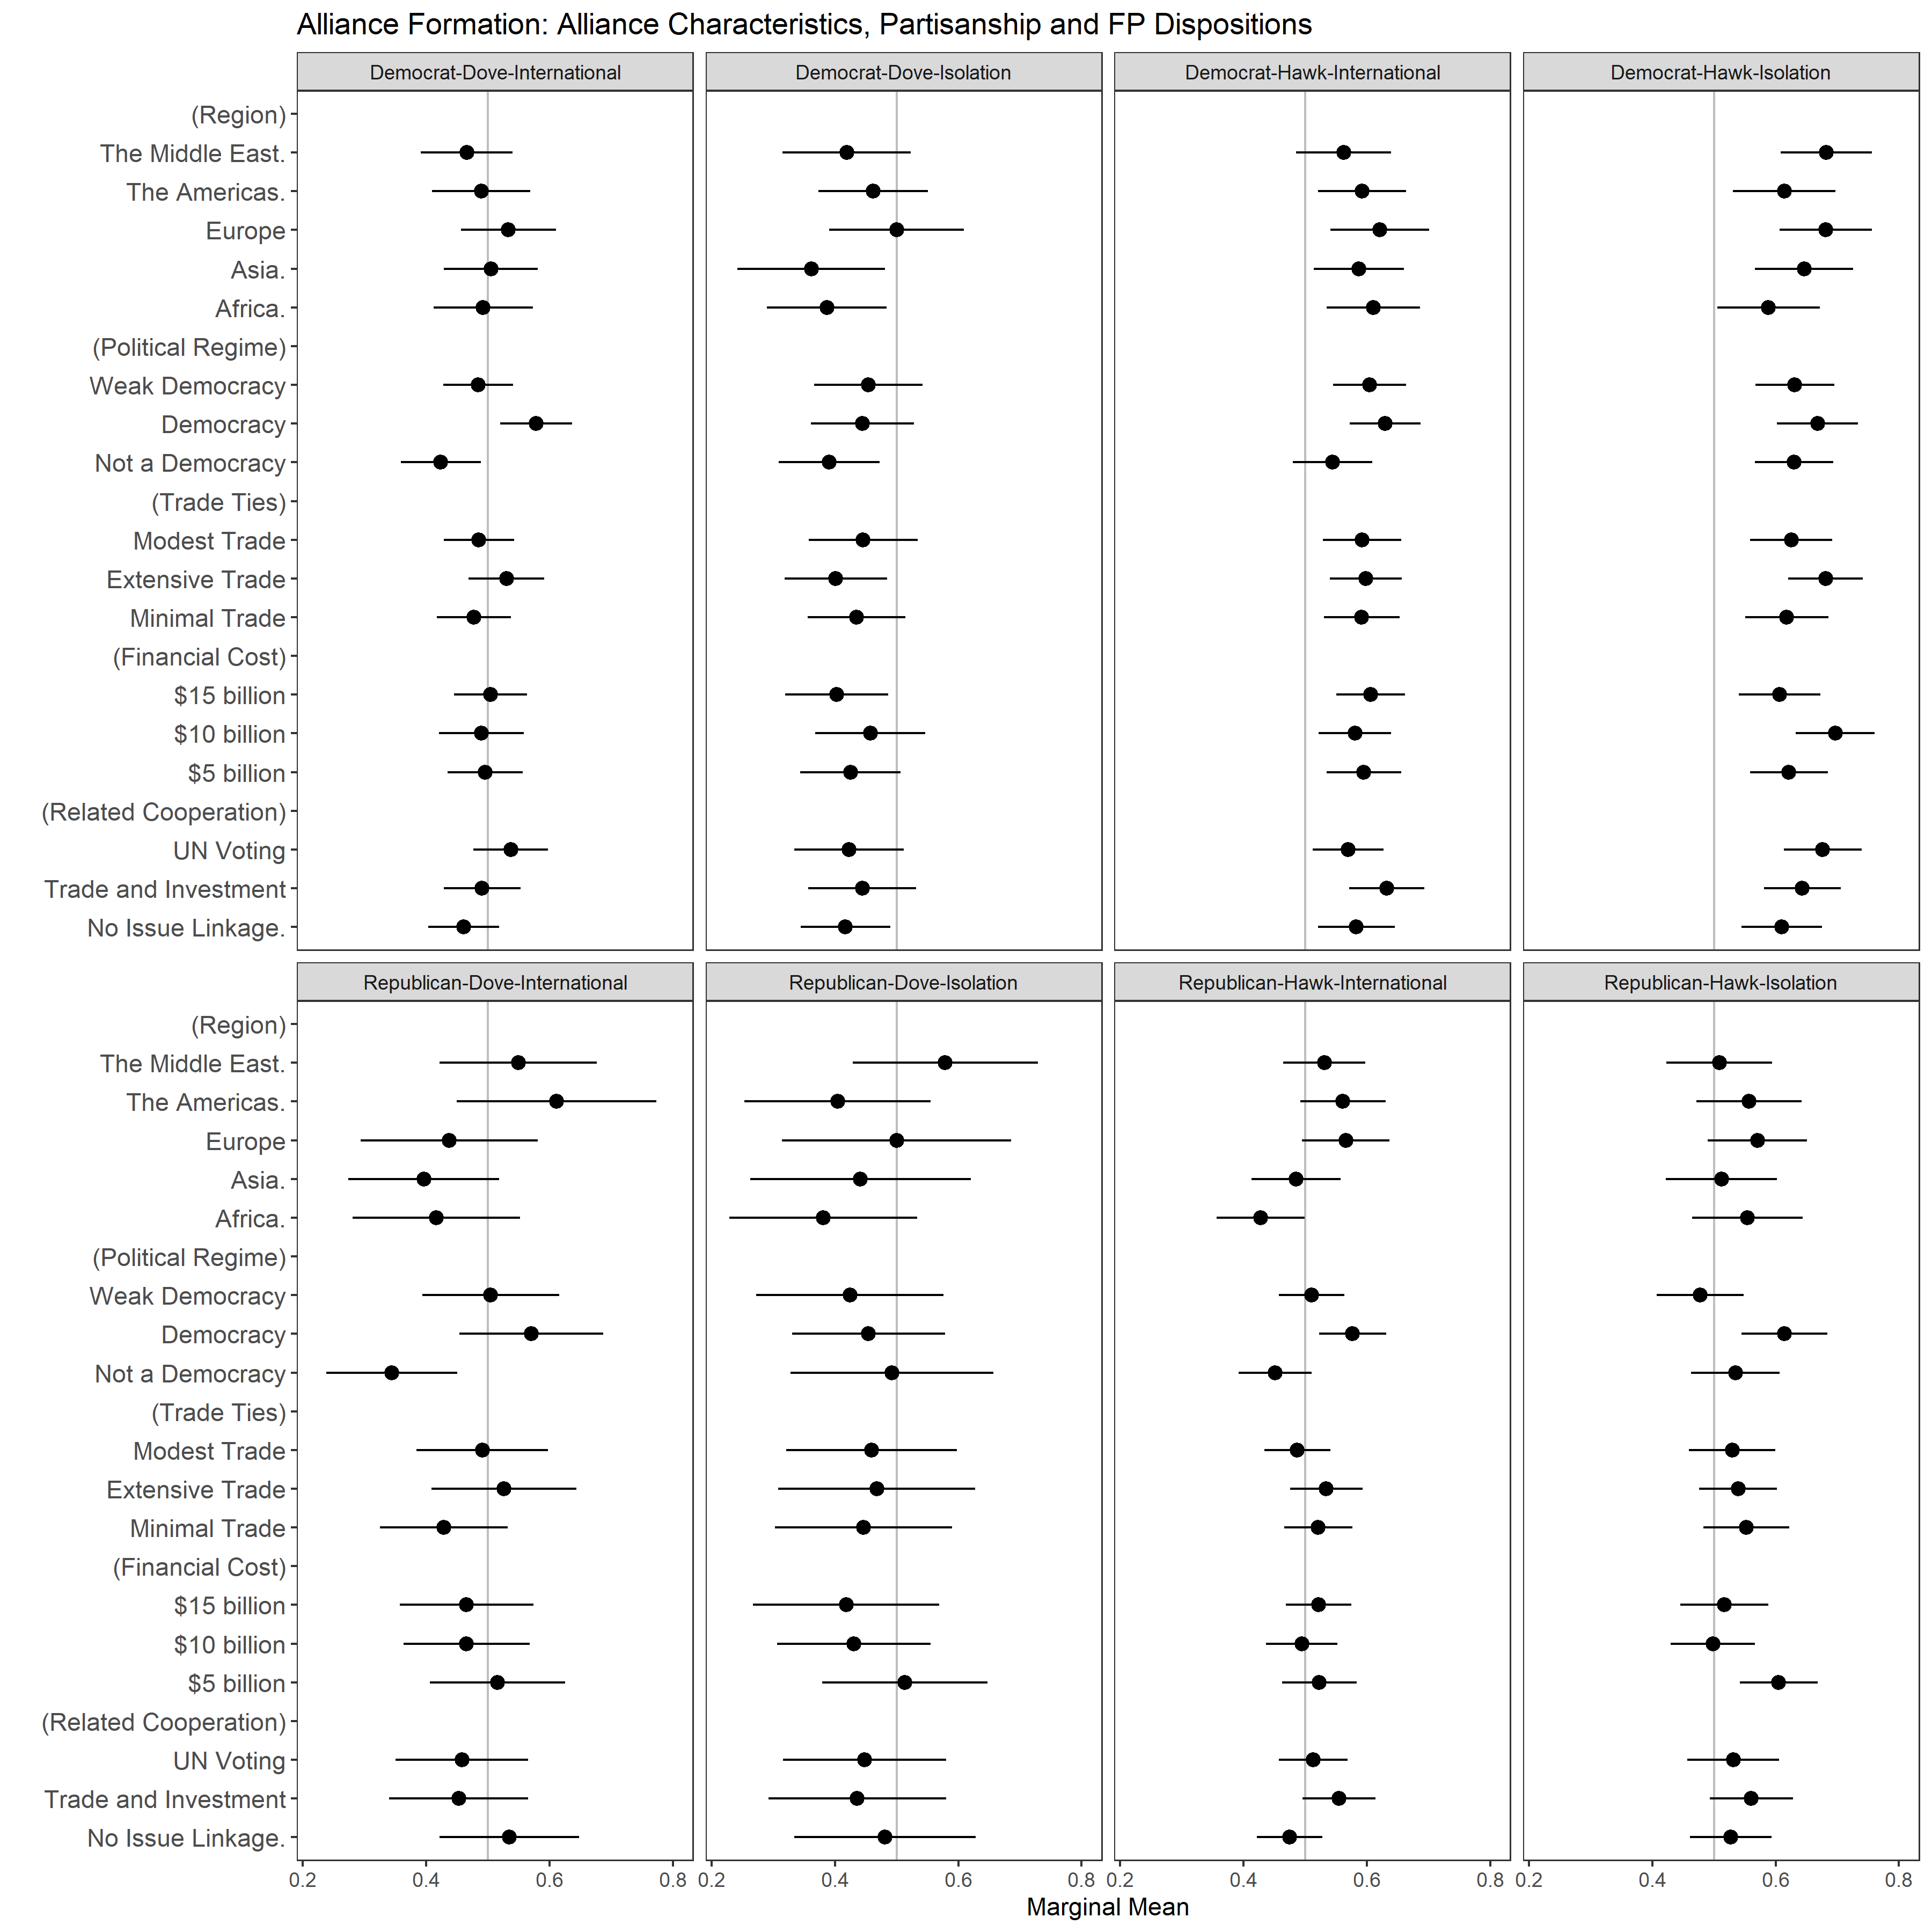
\includegraphics[width=0.95\textwidth]{../figures/party-dispo-form-char.png}
	\caption{Marginal means of support for forming a hypothetical alliances across party identification and foreign policy dispositions under different alliance characteristics. For each group, the estimates mark the marginal mean of support for alliance participation under different alliance treatments. Vertical line highlights a marginal mean of .5, as it is a threshold for majority support. Components marked with abbreviated labels to make the plot more legible. Independents omitted.}
	\label{fig:party-dispo-form-char}
\end{figure}



\begin{figure}
	\centering
		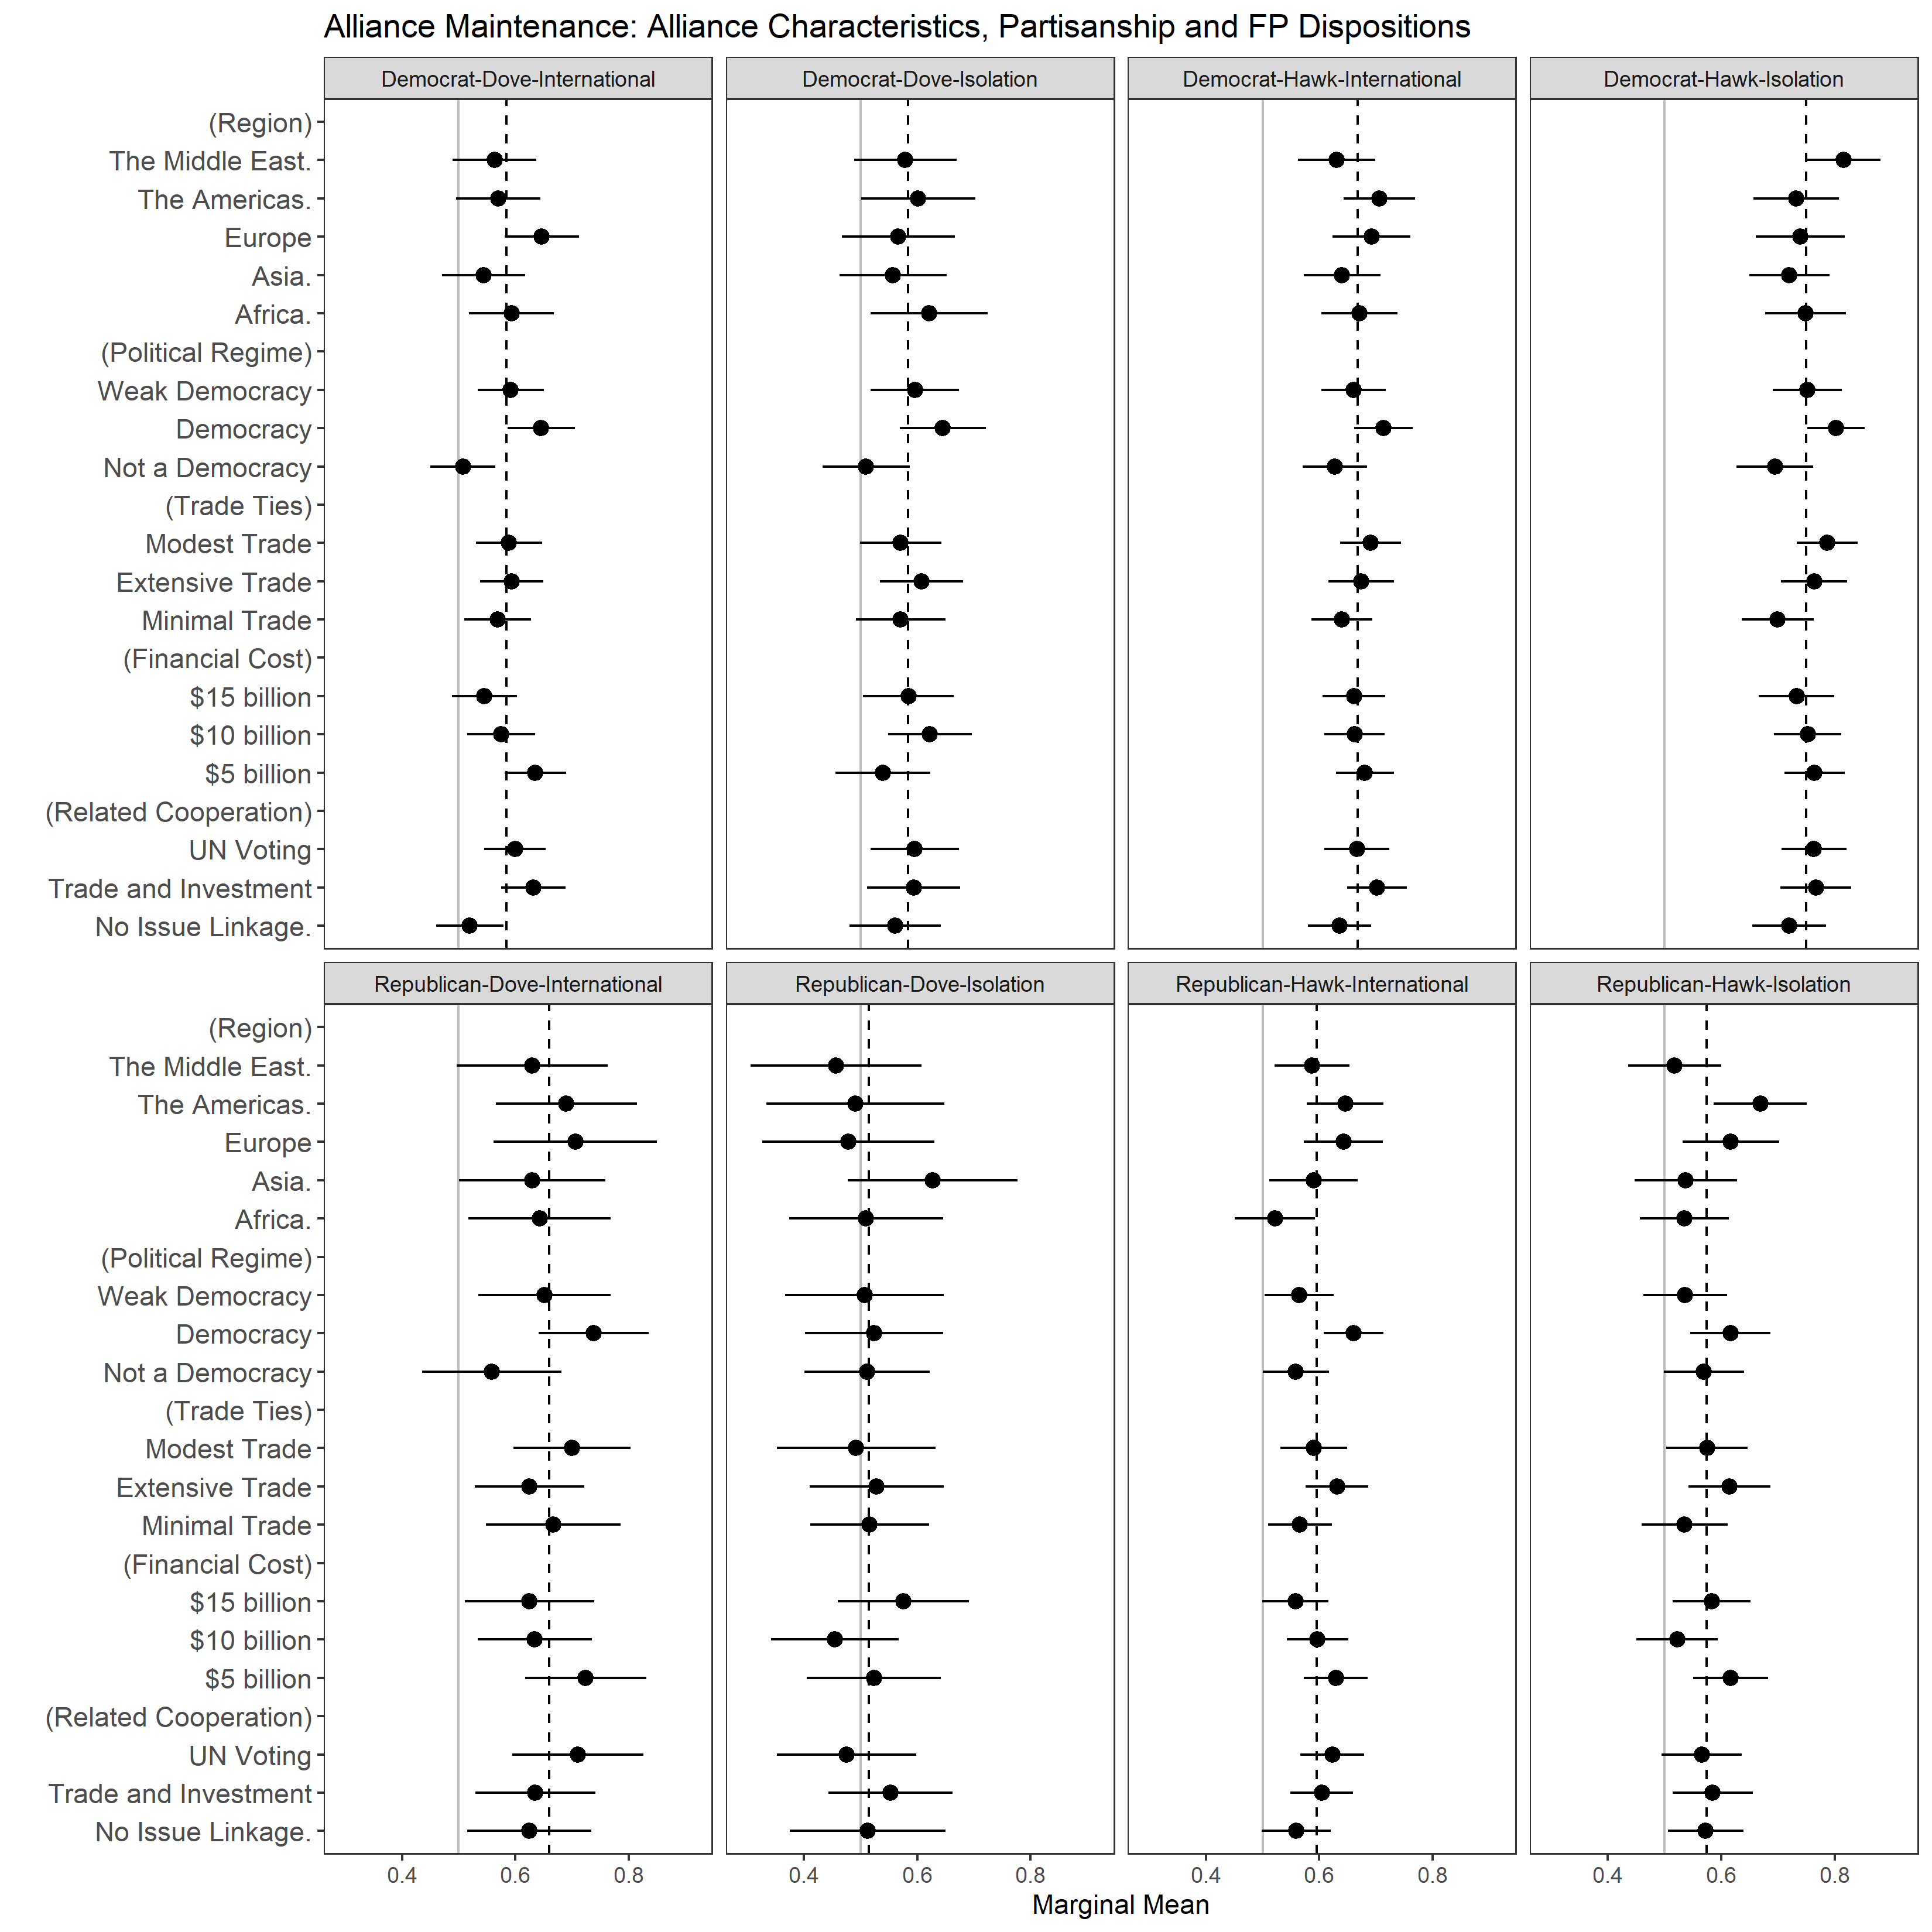
\includegraphics[width=0.95\textwidth]{../figures/party-dispo-main-char.png}
	\caption{Marginal means of support for maintaining a hypothetical alliances across party identification and foreign policy dispositions under different alliance characteristics. For each group, the estimates mark the marginal mean of support for alliance participation under different alliance treatments. Vertical line highlights a marginal mean of .5, as it is a threshold for majority support. Components marked with abbreviated labels to make the plot more legible. Independents omitted.}
	\label{fig:party-dispo-main-char}
\end{figure}



% other differences in region
Both experiments also show partisan differences in attitudes towards alliances in different regions. 
Hawkish Republicans are very skeptical of alliances with African countries. 
Instead, these individuals prefer alliances in Europe or the Americans. 
Democrats with similar foreign policy dispositions express no regional preferences. 


% Some points of consistency
Support for international engagement also produces some partisan overlap in alliance attitudes. 
Internationalist individuals are more responsive to trade and foreign policy issue linkages more than isolationists. 
In the alliance maintenance experiment, dovish and internationalist individuals are also more likely to reduce their support as alliance costs increase. 


% highlight differences in formation and maintenace
All of the above results also show that baseline support for forming new alliances is lower than support for maintaining existing treaties. 
A bare majority of respondents support alliance formation in many circumstances. 
Dovish isolationists are particularly opposed to new alliances, though these Democrats can be convinced by elites. 
Elite cues are especially important for new alliances, as whether elites support or oppose an alliance determines whether it has majority or minority support within each party. 
Regardless of the exact alliance characteristics or elite cues, the marginal means of support for alliance maintenance are almost all above .5. 
Even dovish isolationists are at least roughly divided in support for alliance maintenance.


% wrap up
These results suggest that partisanship and foreign policy dispositions interact to shape alliance attitudes, which are largely a function of elite cues. 
There is an important asymmetry in partisan alliance attitudes and elite cues. 
Democrat elites have some power to lead alliance skeptics, and less influence over committed alliance supporters. 
Republican elites can lead alliance supporters, but have limited influence on committed alliance skeptics. 
As a result, the impact of elite cues depends on individual concerns, but cues exert substantial influence on the majority of both parties. 





\section{Discussion and Conclusion} 

% Overview
I find that elites can lead alliance attitudes, though there are important differences in how individuals respond. 
Partisans respond largely to cues from co-partisan elites, but the magnitude of their response depends on individual hawkishness and isolationism. 
Issue linkages, shared threat, financial cost and trade have a more limited but noticeable  impact as well.  


% thus, net on puzzle
Elites have substantial latitude to lead public opinion on alliances, but individual concerns limit their leadership over certain sections of both parties. 
The most committed alliance supporters ---hawkish isolationist Democrats--- pay less attention to elite cues.
Similarly, elite cues have little impact on the most committed alliance skeptics --- dovish and isolationist Republicans. 
There is therefore a partisan asymmetry in elite leadership of alliance attitudes. 
Republicans can lead alliance supporters, while Democrats can lead alliance skeptics. 


% bring it in on observed alliances
These findings have four key implications for understanding public attitudes towards alliances like NATO. 
First, the Republican and Democratic parties have small but important sets of committed alliance skeptics and supporters, respectively.
Outside these groups and pure independents, most Americans are fairly responsive to elite cues in their alliance attitudes. 
How much elites pander to fixed alliance attitudes in their party is therefore a crucial issue. 
At the same time, elite opposition rarely pushes alliance attitudes into majority opposition to existing treaties. 


Second, allied democracy is crucial to continued public support for alliances.
Many Americans, especially Democrats, dislike alliances with non-democracies. 
Democratic backsliding in U.S. allies could therefore undermine public support for alliances. 


Third, these findings support the view that cycles in public opinion could make democratic commitments less reliable \citep{GartzkeGleditsch2004}. 
Although these results suggest that many members of the public hold considered opinions \citep{PageShapiro1992}, they also show that elites have substantial power to lead. 
One set of elites alone can push aggregate support from a solid majority to a evenly divided issue in their party.
Should military or diplomatic elites ever publicly oppose alliances, they could bolster the impact of skeptical politicians and cut public support. 


% why NATO robust under Trump? 
Finally, these results may help explain public opinion towards alliances like NATO during the Trump administration.
Although Trump often criticized U.S. allies, alliance commitments usually commanded majority support throughout his administration \citep{PewNATO2020}. 
Some of this reflects Democrat's aversion to Trump, but concern that Trump would inspire resurgent isolationism in the Republican party may have been overstated in alliance politics. 
The hawkishness of many Republicans can somewhat offset isolationism in alliance attitudes.
Isolationist and dovish Republicans did not change their alliance attitudes in response to Trump's rhetoric, as it pandered to their views. 


% limitations
These findings have some limitations. 
For one, while the sheer variety of alliances means that the above profiles are plausible, generalizing from survey experiments can be challenging. 
The artificial nature of a survey experiment provides the necessary control to disentangle different sources of public attitudes, but no hypothetical alliance can perfectly reflect real world commitments.


% non-us results- might be different, subject for future inquiry
This study also focuses on the United States, which has an unusual alliance network. 
Though public opinion towards alliances in the United States is important, attitudes in other countries matter as well. 
Future research should examine the sources of alliance attitudes in other countries. 


% future stuff: feedback, content of elite cues
These results provide a foundation for further inquiry into the domestic politics of military alliances. 
Two questions are especially interesting in this respect.
First, how much feedback is there between public opinion and elite cues? 
When might politicians pander to committed alliance supporters or skeptics, or lead the rest of their party in a different direction? 
Politicians might view marginal changes in opinion due to changes in threat or allied democracy as an opportunity to encourage or arrest further changes in public support.
Second, would leaders face significant public disapproval if they withdrew from an alliance? 


These questions speak to the general process by which elites form and maintain domestic coalitions for or against international engagement. 
In the 75 years since the end of World War II, shifting elite cues, partisan attitudes and allied characteristics may mean that different groups back alliances today than in 1950, even when the top line support numbers are similar. 
Tracking changes in the domestic coalitions backing alliances is another worthwhile task for future research.


% wrap it up 
In conclusion, public opinion towards alliances is largely a function of elite cues, but elites cannot lead the whole electorate.  
Important subsets of both parties hold very rigid alliance attitudes. 
Alliances attitudes are therefore a complex mixture of top-down cues and bottom up considerations. 



\newpage

% Bibliography
 
\bibliography{../../MasterBibliography} 




\end{document}
